\chapter{Axiomatizing General Concept Inclusions with High Confidence}
\label{cha:axiom-conf-el}

The results obtained by Distel about computing finite bases of finite interpretations are
not only interesting from a theoretical point of view.  Although we have skipped most of
the details, all the relevant results are \emph{effective} in the sense that the obtained
bases can in principle be computed by computers.  Thus, these results may also be
interesting for practical applications.

A possible application of Distel's results is to compute bases from \emph{Linked Open
  Data}~\cite{Linked-Data}, a format for representing data as used by the semantic
web~\cite{journal/sciam/BernersLeeHL01,DBLP:conf/dagstuhl/2003sweb,FOST}.  This data
format is mainly constituted of RDF triples and can be thought of as an edge-labeled
graph.  As such, it is very similar to interpretations, and thus Distel's results are
applicable here.

As a first contribution of this thesis we have implemented the major results obtained by
Distel on computing finite bases as described previously, and applied them to a particular
data set of the \emph{Linked Open Data Cloud}, namely to a subset of the DBpedia data
set~\cite{DBpedia}.  In \Cref{sec:computing-bases-from} we describe this experiment in
detail and show what Distel's results yield when applied to this data set.  This
experiment has also been discussed previously
in~\cite{Borchmann:confident-GCIs,DBLP:conf/icdm/BorchmannD11}.

One conclusion from this experiment is that Distel's results are very sensitive to
\emph{errors} in the data.  This is actually not surprising: bases of finite
interpretations only contain general concept inclusion which are valid in the data, and if
there is only one single counterexample to a general concept inclusions, it will not be
contained in any base.

If those counterexamples are erroneous, however, then this can cause problems.  Not only
that otherwise valid general concept inclusions are not obtained by Distel's approach
anymore.  Sporadic erroneous counterexamples may also cause GCIs found during the
computation of bases to be rather complicated, because those GCIs have to avoid those
erroneous counterexamples.

To remedy, or at least to alleviate this effect of erroneous counterexample to computing
finite bases we shall consider an extension of Distel's results which tries to find bases
of GCIs which are not necessarily valid in the given interpretation, but instead enjoy a
\emph{high confidence} in it.  The notion of \emph{confidence} is borrowed from
data-mining~\cite{arules:agrawal:association-rules}, more precisely from the theory of
\emph{association rules}, and allows to measure how much an association rule is allowed to
ignore counterexamples.  We shall transfer the notion of confidence to general concept
inclusions, and shall then try to find bases for those \emph{GCIs with high confidence}.

For this we shall make use of results obtained by Luxenburger from his work on
\emph{partial implications}~\cite{diss:Luxenburger,Luxenburger91}, and extensions
thereof~\cite{DBLP:conf/ki/StummeTBPL01}.  Partial implications can be thought of as
implications considered together with their confidence in some particular formal context.
We shall discuss in \Cref{Luxen-base} how these results allow us to obtain bases of all
implications which have \emph{high confidence} in some given formal context.

In \Cref{sec:first-base} we then show how these ideas can be simulated in \ELgfpbot to
find bases for GCIs with high confidence.  Moreover, we shall also show in
\Cref{sec:bases-confident-gcis} how bases of implications with high confidence yield bases
of GCIs with high confidence.  Finally, we shall also discuss a way to \emph{complete}
sets of GCIs, \ie how to obtain a set of valid GCIs that makes a given set of GCIs
complete.  This result is quite similar to \Cref{thm:Felix-base-B3}, and we shall do this
in \Cref{sec:completing-sets-of-gcis}.  Finally, we shall see how to obtain \ELbot bases
from \ELgfpbot bases for GCIs with high confidence.

The results thus obtained are again all effective, and we shall discuss some experiments
in \Cref{sec:exper-with-conf} which use the same data-set as the one used in
\Cref{sec:computing-bases-from}.  This allows us to directly compare the approaches of
computing bases of valid GCIs on the one hand, and bases of GCIs with high confidence on
the other.  Moreover, we shall also discuss shortcomings of the approach of considering
GCIs with high confidence, which will eventually lead us to considering extensions of the
attribute exploration algorithm.  These will be discussed in \Cref{cha:expl-conf} and
\Cref{cha:model-expl-conf}.

\section{Computing Bases from DBpedia}
\label{sec:computing-bases-from}

We want to evaluate the practicability of Distel's results by applying them to linked data
extracted from the Linked Open Data Cloud.  In other words, given some linked data, we
want to extract a complete set of general concept inclusions that is valid within this
data set.  The goal of this experiment is to see in how far Distel's approach is practical
in learning terminological knowledge about some domain which is represented by linked data.

Of course, before we can do so we first have to discuss how we can obtain an
interpretation from a given linked data set, and one which sufficiently reflects the
logical structure of the initial data set.

Recall that a finite interpretation $\mathcal{I} = (\Delta^{\mathcal{I}},
\cdot^{\mathcal{I}})$ over $N_C$ and $N_R$ consists of a set $\Delta^{\mathcal{I}}$ and a
mapping $\cdot^{\mathcal{I}}$ that maps every $A \in N_C$ to a set $A^{\mathcal{I}}
\subseteq \Delta^{\mathcal{I}}$, and every $r \in N_R$ to a set of pairs $r^{\mathcal{I}}
\subseteq \Delta^{\mathcal{I}} \times \Delta^{\mathcal{I}}$.  We have also already seen
some examples of depicting interpretations as \emph{graphs}, more precisely as
\emph{directed edge- and vertex-labeled graphs}.  Indeed, interpretations are essentially
nothing else than those graphs, where the set of vertex labels is $N_C$ and the set of
edge labels is $N_R$.

Linked data is now quite similar to labeled graphs.  More precisely, linked data is just
an edge-labeled graph, represented by so-called \emph{RDF-Triples}.  Every triple consists
of a \emph{subject}, a \emph{predicate}, and an \emph{object} (in that order), each of
them being an \emph{uniform resource identifier} (URI).  The idea is that RDF-Triples
encode the information that the subject is connected to the object by means of the
predicate.  Two examples of RDF-Triples, taken from the DBpedia data set~\cite{DBpedia},
are\footnote{Indeed, these are \emph{serializations} of RDF-Triples, in this case in the
  so-called \emph{N-Triples} format}
\begin{verbatim}
  <http://dbpedia.org/resource/Aristotle>
  <http://www.w3.org/1999/02/22-rdf-syntax-ns#type>
  <http://dbpedia.org/ontology/Philosopher> .

  <http://dbpedia.org/resource/Aristotle>
  <http://dbpedia.org/ontology/influenced>
  <http://dbpedia.org/resource/Western_philosophy> .
\end{verbatim}
Intuitively, these triples encode the facts that \emph{Aristotle is (was) a philosopher}
and that \emph{Aristotle influenced Western Philosophy}.

Since RDF-Triples constitute edge-labeled graphs, we can take them as they are and regard
them as interpretations over $N_C = \emptyset$ and $N_R$, where $N_R$ is just the set of
all predicates which appear in RDF-Triples in the data set.  This approach would work,
however it would only yield GCIs where no concept names are present.  Such terminological
knowledge may not be very interesting.

To alleviate this problem we make use of the special RDF predicate
\begin{equation}
  \label{eq:16}
  \verb|http://www.w3.org/1999/02/22-rdf-syntax-ns#type|
\end{equation}
which expresses that a subject is an instance of a certain
class.\footnote{\url{http://www.w3.org/1999/02/22-rdf-syntax-ns}} If we consider triples
with this predicates not as edges in the linked graph, but instead as the information that
the subject is an instance of the object, then we indeed consider linked data as a vertex-
and edge-labeled graph with vertex labels $N_C$ and edge-labels $N_R$, where $N_C$ is not
empty in general.

This view on linked data now allows us to consider it as an interpretation over some sets
$N_C$ and $N_R$, and to apply Distel's result to such data sets.  For our experiments, we
have chosen a subset of the DBpedia data set as of March 2010 (Version
3.5)\footnote{\url{http://wiki.dbpedia.org/Downloads35?v=pb8}}.  The linked data contained
within the DBpedia data-set has been extracted automatically from \emph{Wikipedia
  Infoboxes}, which are a means to represent facts about the topic of the current page in
a compact way.

\begin{figure}[tp]
  \centering
  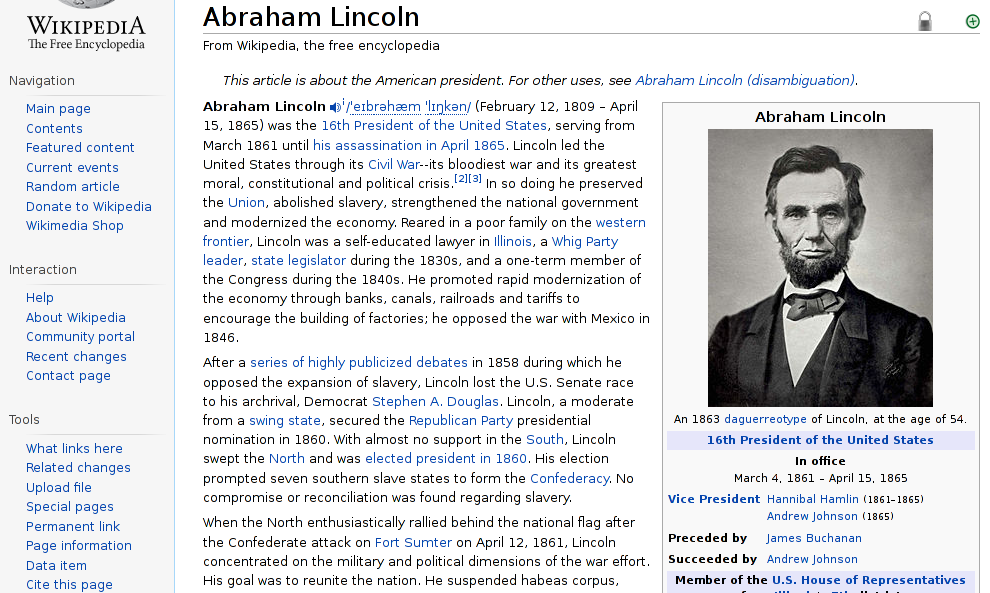
\includegraphics[width=20em]{chapters/lincoln-infobox.png}
  \caption{Wikipedia Article about Abraham Lincoln with Infobox on its Right}
  \label{fig:infobox-screenshot}
\end{figure}

The subset of the DBpedia data-set we used for our experiments arises by restricting our
attention to the relation
\begin{equation*}
  \verb|http://dbpedia.org/ontology/child|.
\end{equation*}
From this subset, we constructed an interpretation $\Idbpedia = (\Delta^{\Idbpedia},
\cdot^{\Idbpedia})$.  To make the following considerations easier to read we shall drop
the prefix and just write \textsf{child} instead of
\texttt{http://dbpedia.org/ontology/child}, for example.

To construct $\Idbpedia$ we first computed all triples $T_{\mathsf{child}}$ from the
DBpedia data set whose predicate is \textsf{child}.  The subjects of these triples where
collected into $\Delta^{\Idbpedia}$.  We defined
\begin{equation*}
  \mathsf{child}^{\Idbpedia} := \set{ (s, o) \in \Delta^\Idbpedia \times \Delta^\Idbpedia
    \mid (s, \mathsf{child}, o) \in T_{\mathsf{child}} }.
\end{equation*}
Examples for triples contained in $T_{\mathsf{child}}$ are
\begin{verbatim}
  <Abraham_Lincoln> <child> <Robert_Todd_Lincoln> .
  <Abraham_Lincoln> <child> <Edward_Baker_Lincoln> .
\end{verbatim}
Therefore,
\begin{align*}
  (\mathsf{Abraham\_Lincoln}, \mathsf{Robert\_Todd\_Lincoln}) &\in \mathsf{child}^{\Idbpedia},\\
  (\mathsf{Abraham\_Lincoln}, \mathsf{Edward\_Baker\_Lincoln}) &\in \mathsf{child}^{\Idbpedia}.
\end{align*}

Then we considered all triples $T_{\mathsf{type}}$ whose predicate is the special type
predicate of \Cref{eq:16} and whose subject is contained in $\Delta^{\Idbpedia}$.  The
objects of those triples where collected into a set $N_C$, \ie they constituted the
concept names of $\Idbpedia$.\footnote{We omitted
  \texttt{http://www.w3.org/2002/07/owl\#Thing} in $N_C$, as it does not introduce any
  meaningful information} Then, for an $A \in N_C$, we defined $A^{\Idbpedia}$ to be the
set of all subjects which appear in a triple in $T_{\mathsf{type}}$, \ie
\begin{equation*}
  A^{\Idbpedia} := \set{ s \in \Delta^{\Idbpedia} \mid (s, t, A) \in
    T_{\mathsf{type}} }
\end{equation*}
where $t$ stands for the special RDF type predicate of \Cref{eq:16}.  Example triples from
$T_{\mathsf{type}}$ concerning \verb|Abraham_Lincoln| are
\begin{verbatim}
  <Abraham_Lincoln>
  <http://www.w3.org/1999/02/22-rdf-syntax-ns#type>
  <Person> .

  <Abraham_Lincoln>
  <http://www.w3.org/1999/02/22-rdf-syntax-ns#type>
  <OfficeHolder> .
\end{verbatim}
and therefore
\begin{align*}
  \mathsf{Abraham\_Lincoln} &\in \mathsf{Person}^{\Idbpedia}, \\
  \mathsf{Abraham\_Lincoln} &\in \mathsf{OfficeHolder}^{\Idbpedia}.
\end{align*}

The interpretation $\Idbpedia$ then 5624 elements and contained 60 concept names, \ie
$\abs{ N_C } = 60$.  By construction, that there is only one role name in $\Idbpedia$,
namely \textsf{child}.  To now compute bases of $\Idbpedia$ means to extract all knowledge
about the child-relation present in DBpedia and expressible in \ELbot.  Note that elements
from DBpedia are only present in $\Idbpedia$ if they have children, or are children of
someone else.  Moreover, as DBpedia extracts its information from Wikipedia, all elements
in $\Idbpedia$ correspond to articles in Wikipedia; in particular, if such elements
correspond to persons, then those persons have to be ``sufficiently famous'' in the sense
that they deserve a Wikipedia article.  Therefore, $\Idbpedia$ represent DBpedia's
knowledge about famous persons and their famous children.

We have to note, however, that the \emph{child}-relation in DBpedia contains some false
information, mostly due to the way this information is extracted from Wikipedia Infoboxes.
More precisely, our interpretation $\Idbpedia$ not only contains elements which correspond
to humans, but also contains elements which are instances of \textsf{Work},
\textsf{Organisation} or \textsf{PopulatedPlace}, among others.  However, those artifacts
are comparably rare, and it is still reasonable to use $\Idbpedia$ for our experiments.

We have implemented the algorithms devised by Distel to compute bases of finite
interpretations\footnote{\url{http://github.com/exot/EL-exploration}} on top of
\texttt{conexp-clj}\footnote{\url{http://github.com/exot/conexp-clj}}, a general purpose
tool for formal concept analysis.  When computing a minimal base of $\Idbpedia$ as
described in \Cref{thm:Felix-5.18}, we obtained a base $\mathcal{B}_{\Idbpedia}$
containing 1252 general concept inclusions.  In the following we want to examine the GCIs
contained in this bases, describe some observations we made, and discuss the usefulness of
these GCIs.  Of course, we cannot do this formally, and shall therefore only argue
intuitively.

Firstly, some of the GCIs contained in $\mathcal{B}_\Idbpedia$ constitute knowledge about
the relationships among the concept names occurring in $\Idbpedia$ only, for example
\begin{align*}
  \sf Politician &\sqsubseteq \sf Person \\
  \sf MemberOfParliament &\sqsubseteq \sf Person \sqcap Politician \\
  \sf Criminal \sqcap Politician &\sqsubseteq \bot
\end{align*}
This knowledge can indeed be useful to learn the hierarchy of concept names
(\emph{taxonomy}) of $\Idbpedia$.  On the other side, this knowledge does not yet show
whether Distel's results are useful, as this knowledge could have easily been obtained my
methods from formal concept analysis alone.

The last GCI states that there are no elements in $\Idbpedia$ that are both criminal and
politicians.  GCIs of this form are called \emph{disjointness constraints}, and they can
be useful in applications.  The disjointness constraint shown above only contain concept
names.  However, Distel's approach let's us find more disjointness constraints than just
between concept names.  For example, $\mathcal{B}_{\Idbpedia}$ contains the GCI
\begin{equation*}
   \sf Philosopher \sqcap \exists child. \top \sqsubseteq \bot
\end{equation*}
expressing that philosophers don't have children (or at least not children famous enough
to occur in Wikipedia).  Indeed, since $\mathcal{B}_{\Idbpedia}$ is complete for
$\Idbpedia$, all disjointness constraints valid in $\Idbpedia$ can either be found in this
base or are entailed by it.  Such information can be of practical relevance.

There are other GCIs contained in $\mathcal{B}_\Idbpedia$ which are not disjointness
constraints or only express knowledge about concept names.  Two of them for which we could
argue that they can be useful are
\begin{align*}
  \sf \exists child. Person &\sqsubseteq \sf Person, \\
  \sf FictionalCharacter \sqcap \exists child. Person &\sqsubseteq \sf \exists child. FictionalCharacter
\end{align*}
where the second GCI can be seen as some kind of \ELbot approximation of the fact that
fictional characters can only have fictional characters as their children.  These GCIs can
indeed be seen as useful terminological knowledge for the domain represented by
$\Idbpedia$.

Those GCIs, \ie where one could argue that they represent meaningful knowledge, are quite
rare in $\mathcal{B}_\Idbpedia$.  On the other hand, $\mathcal{B}_\Idbpedia$ contains many
GCIs whose usefulness is highly doubtful, either because they combine otherwise unrelated
concepts, or they are too specific.

An example for the first case is
\begin{equation*}
  \sf Person \sqcap \exists child. Book \sqsubseteq FictionalCharacter
\end{equation*}
which does not really represent any meaningful knowledge.  On the other hand, this GCI
indicates that DBpedia finds books as children only on Wikipedia pages on fictional
characters.  Thus, such GCIs may help to find errors in the way DBpedia extracts
information, but are not helpful as knowledge itself.  Similar examples are
\begin{align*}
  \sf \exists child. Newspaper \sqcap Person &\sqsubseteq \sf Writer, \\
  \sf \exists child. MilitaryUnit &\sqsubseteq \sf Judge, \\
  \sf \exists child. Settlement \sqcap Politician &\sqsubseteq \sf Congressman.
\end{align*}

GCIs which could be too specific can be considered to most common case among all GCIs in
$\mathcal{B}_{\Idbpedia}$, examples of them being
\begin{gather*}
  \sf \exists child. Ambassador \sqcap OfficeHolder \\
  \sqsubseteq \sf \exists child. (Ambassador \sqcap \exists child. Person) \sqcap {}\\
  \phantom{\sqsubseteq{}} \sf\exists child. (OfficeHolder \sqcap \exists child.
  Congressman \sqcap \exists child. Actor \sqcap \exists child OfficeHolder).
\end{gather*}
Indeed, this GCI only applies to the individual \texttt{Joseph\_P.\_Kennedy\%2C\_Sr.}, and
thus it states information only about this very individual and its children.  To cope with
such situations, Distel extended his results about computing bases of finite
interpretations to \emph{model exploration} which also allows for \emph{expert
  interaction}, in a way similar to attribute exploration in formal concept analysis.  If
the expert would encounter such a GCI she would reject it as being too specific, and would
provide more examples to make it more general.  We shall discuss this algorithm in more
detail in \Cref{cha:model-expl-conf}.

Another approach to eliminating those over-specific GCIs may be to require for the
extracted GCIs that they apply to at least a certain number of different individuals.
However, this approach leads to some unintuitive behavior, see \Cref{cha:conclusions}.

Finally, among the GCIs contained in $\mathcal{B}_\Idbpedia$ there exist some which convey
the impression of being redundant, like
\begin{equation*}
  \sf \exists child. \exists child. \top \sqsubseteq \exists child. (Person \sqcap \exists child. \top),
\end{equation*}
because it should be quite clear from the construction of $\Idbpedia$ that only persons
can have children, \ie the following GCI
\begin{equation}
  \label{eq:23}
  \sf \exists child. \top \sqsubseteq Person
\end{equation}
should hold in $\Idbpedia$.  This is because only Wikipedia articles of human beings
should contain a child-entry within their Infobox.  Thus, even with all the errors in
$\Idbpedia$ concerning non-persons that we have discussed before, the GCI in \Cref{eq:23}
should hold in $\Idbpedia$.

However, this is not the case, since there are four counterexamples to this GCI in
$\Idbpedia$, \ie elements $x \in \Delta^{\Idbpedia}$ satisfying $x \in (\sf \exists
child. \top)^{\Idbpedia} \setminus Person^{\Idbpedia}$.  These
are\footnote{Coincidentally, all these are artists from Hong Kong}
\begin{equation*}
  \mathtt{Teresa\_Carpio},\; \mathtt{Charles\_Heung},\;
  \mathtt{Adam\_Cheng}, \; \mathtt{Lydia\_Shum}.
\end{equation*}
However, these elements clearly represent human beings, so they \emph{should} actually be
instances of \textsf{Person}.  In other words, these counterexamples are all
\emph{erroneous} counterexamples, but since they are present in $\Idbpedia$ the approach
developed by Distel will not ignore them.  This not only inhibits finding the GCI $\sf
\exists child. \top \sqsubseteq Person$, but also causes incomprehensible GCIs to be
found which are special cases of this GCI but somehow try to ``circumvent'' the erroneous
counterexamples. An example for this is
\begin{gather*}
  \sf Person \sqcap \exists child. (Person \sqcap \exists child. (Person \sqcap \exists child.
  (Person \sqcap {}\\
  \quad \quad \sf \exists child. \exists child. (Person \sqcap \exists child. \top))))
  \\
  \sf \quad \sqsubseteq
  \exists child. (Person \sqcap \exists child. (Person \sqcap \exists child. (Person \sqcap
  \exists child. (Person \sqcap {}\\
  \sf \quad \quad \exists child. \exists child. Person)))).
\end{gather*}

\section{GCIs with High Confidence in Finite Interpretations}
\label{sec:confident-gcis}

It would certainly increase the applicability of Distel's approach if we could ignore
erroneous counterexamples in our data, as then we could expect simpler and more general
GCIs to be extracted.  However, we cannot expect to have an automatic procedure which
achieves this goal, \ie we cannot expect an algorithm that automatically ignores erroneous
counterexamples, since the algorithm would need to know what errors are in the current
domain of interest, and for this the algorithm would need to posses knowledge about this
domain, which however we are just about to learn.

On the other hand, what we can assume is that our initially given interpretation
$\mathcal{I}$ contains only \emph{few} errors, as otherwise learning GCIs from it would be
futile.  Based on this assumption we can approach the problem of erroneous counterexamples
as follows: if it is the case that $\mathcal{I}$ contains much more \emph{positive
  examples} for a GCI $C \sqsubseteq D$ than \emph{negative} ones, then we assume that the
negative counterexamples are ``probably erroneous.''  Here, a \emph{positive example} for
$C \sqsubseteq D$ would be an element $x \in \Delta^{\mathcal{I}}$ satisfying $x \in
C^{\mathcal{I}} \cap D^{\mathcal{I}}$, and a \emph{negative example} for $C \sqsubseteq D$
would be an element $y \in \Delta^{\mathcal{I}}$ such that $y \in C^{\mathcal{I}}
\setminus D^{\mathcal{I}}$.  We can consider a GCI to be ``almost valid'' in $\mathcal{I}$
if the number of positive examples is much higher than the number of negative ones.  The
approach to ignore erroneous counterexamples would then be to consider these ``almost
valid'' GCIs in addition to the valid ones, and try to find finite bases for both of them.

This actually works quite well for our example interpretation $\Idbpedia$, as the GCI $\sf
\exists child. \top \sqsubseteq Person$ has much more positive than negative examples:
there are 2551 elements $x \in \Delta^{\Idbpedia}$ to which $\sf \exists child. \top
\sqsubseteq Person$ applies, \ie which satisfy $x \in (\sf \exists child. \top)$, but only
4 of those (the ones mentioned above) fail to also satisfy $x \in \sf Person^{\Idbpedia}$.
Therefore, $\sf \exists child. \top \sqsubseteq Person$ has 2547 positive examples, but
only 4 negative ones.  By our approach, we can consider these negative examples as errors
and ignore them.  Thus, $\sf \exists child. \top \sqsubseteq Person$ would be extracted
from $\Idbpedia$.

Of course, this approach is highly heuristic in general: if valid counterexamples for a
GCI $C \sqsubseteq D$ are just \emph{rare} in $\mathcal{I}$, then the above sketched
approach would treat them as errors, which is incorrect.  On the other hand, it may be
much more desirable to extract GCIs which are \emph{wrong} in some application domain,
than to miss GCIs which are \emph{correct}, as long as not too many wrong GCIs are being
extracted.  This is because identifying wrong GCIs can be considered much easier than
finding correct GCIs that are just invalidated by errors in the data.

It is the purpose of this section to give a formalization of the notion of a GCI to be
``almost valid'' in some finite interpretation.  We shall base this formalization on the
notion of \emph{confidence} as it is used in
data-mining~\cite{arules:agrawal:association-rules}.  This will be done in
\Cref{sec:conf-gcis-conf}.  Our goal is then to find \emph{finite bases} of all GCIs which
enjoy a \emph{high confidence} in the initially given interpretation.

\subsection{Confidence of GCIs and Confident Bases}
\label{sec:conf-gcis-conf}

We want to formalize the notion of a GCI $C \sqsubseteq D$ to be ``almost valid'' in some
given interpretation $\mathcal{I}$.  For this we argued intuitively that the number of
positive examples should be ``much higher'' then the number of negative examples.  For
this, we define the \emph{confidence} of $C \sqsubseteq D$ in $\mathcal{I}$.

\begin{Definition}[Confidence of GCIs]
  \label{def:gci-confidence}
  Let $\mathcal{I} = (\Delta^{\mathcal{I}}, \cdot^{\mathcal{I}})$ be a finite
  interpretation over $N_C$ and $N_R$, and let $C, D \in \ELgfpbot(N_C, N_R)$.  Then the
  \emph{confidence} of $C \sqsubseteq D$ in $\mathcal{I}$, written as
  $\conf_{\mathcal{I}}(C \sqsubseteq D)$, is defined as
  \begin{equation*}
    \conf_{\mathcal{I}}( C \sqsubseteq D ) =
    \begin{cases}
      1 & C^{\mathcal{I}} = \emptyset \\
      \frac{\abs{ (C \sqcap D)^{\mathcal{I}} }}{\abs{ C^{\mathcal{I}} }} & \text{otherwise.}
    \end{cases}
  \end{equation*}
\end{Definition}
Note that $(C \sqcap D)^{\mathcal{I}}$ is just the number of positive examples for $C
\sqsubseteq D$ in $\mathcal{I}$, and that $\abs{C^{\mathcal{I}}}$ is just the number of
all elements to which $C \sqsubseteq D$ applies, \ie the number of all positive and
negative examples.  Therefore, $\conf_{\mathcal{I}}(C \sqsubseteq D)$ measures the amount
of positive examples against the number of all elements to which $C \sqsubseteq D$
applies: the higher the confidence of $C \sqsubseteq D$ in $\mathcal{I}$, the more the
number of positive examples is higher than the number of negative ones.

\begin{Example}
  \label{expl:Idbpedia-confidence}
  Recall that $\sf \exists child. \top \sqsubseteq Person$ has 2547 positive and 4
  negative examples in $\Idbpedia$, thus
  \begin{equation*}
    \conf_\Idbpedia( {\sf \exists child. \top \sqsubseteq Person } ) = \frac{ 2547 }{ 2551 }.
  \end{equation*}
\end{Example}

To use the confidence of GCIs in finite interpretations to formalize the notion of being
``almost true'' we need to choose a \emph{threshold} above which we can say that the
number of positive examples is ``much higher'' then the number of negative ones.

\begin{Definition}[Confidence-Based Theory of Finite Interpretations]
  \label{def:confident-theory-of-interpretations}
  Let $\mathcal{I}$ be a finite interpretation over $N_C$ and $N_R$, and let $c \in [0,
  1]$.  Then the \emph{confidence-based theory} of $\mathcal{I}$ \emph{with threshold $c$}
  is defined to be the set
  \begin{equation*}
    \Th_c(\mathcal{I}) := \set{ C \sqsubseteq D \mid C, D \in \ELgfpbot(N_C, N_R),
      \conf_{\mathcal{I}}( C \sqsubseteq D ) \ge c }.
  \end{equation*}
  We say that GCIs in $\Th_c(\mathcal{I})$ have \emph{high confidence} (with respect to
  the threshold $c$).  Sometimes, we may call the elements of $\Th_c(\mathcal{I})$ just
  \emph{confident GCIs}.
\end{Definition}

Note that in general the set $\Th_c(\mathcal{I})$ is not closed under entailment; we shall
see examples for this later on.

Note that if $C \sqsubseteq D$ has confidence 1 in $\mathcal{I}$ if and only if $C
\sqsubseteq D$ holds in $\mathcal{I}$.  Therefore, $\Th(\mathcal{I}) \subseteq
\Th_c(\mathcal{I})$, and thus the set $\Th_c(\mathcal{I})$ is also infinite in general
(\ie when $N_R \neq \emptyset$).  Therefore, we again want to find \emph{finite bases},
this time of the set $\Th_c(\mathcal{I})$.  Recall that a set $\mathcal{B}$ of general
concept inclusions is a base of $\Th_c(\mathcal{I})$ if it is sound and complete for
$\Th_c(\mathcal{I})$, \ie if all GCIs in $\mathcal{B}$ are entailed by
$\Th_c(\mathcal{I})$ and vice versa.

Notice, however, that since $\Th_c(\mathcal{I})$ is not closed under entailment it may
happen that $\mathcal{B} \not\subseteq \Th_c(\mathcal{I})$.  On the other hand it may be
desirable to have bases $\mathcal{B}$ of $\Th_c(\mathcal{I})$ where the GCIs contained in
this base have high confidence as well, \ie which satisfy $\mathcal{B} \subseteq
\Th_c(\mathcal{I})$.  We shall call such bases \emph{confident bases} of
$\Th_c(\mathcal{I})$.

\subsection{Luxenburger's Base}
\label{Luxen-base}

Before we consider finite bases and finite confident bases of $\Th_c(\mathcal{I})$ let us
first consider the analogous problem in formal concept analysis, which is to find small
bases of \emph{implications with high confidence} in a given formal context.  The results
which are relevant for this discussion mainly go back to research done by Luxenburger on
\emph{partial implications}~\cite{diss:Luxenburger,Luxenburger91}.  We shall first discuss
these results, however not in their original form, but instead in way suitable for our
considerations.

We have already defined the notion of confidence of a GCI in some given finite
interpretation.  The analogous notion in formal concept analysis is the confidence of an
implication in a formal context.

\begin{Definition}[Confidence of Implications]
  \label{def:confidence-of-implications}
  Let $\con K = (G, M, I)$ be a finite formal context, and let $(A \to B) \in \Imp(M)$.
  Then the \emph{confidence} of $A \to B$ in $\con K$ is defined as
  \begin{equation*}
    \conf_{\con K}(A \to B) :=
    \begin{cases}
      1 & A' = \emptyset \\
      \frac{ \abs{ (A \cup B)' } } { \abs{ A' } } & \text{otherwise}.
    \end{cases}
  \end{equation*}
\end{Definition}

We can now consider an implication to have \emph{high confidence} in a formal context if
and only if it is above a certain threshold $c \in [0,1]$.

\begin{Definition}[Confidence-Based Theory of Finite Formal Contexts]
  \label{def:theory-with-threshold-for-formal-contexts}
  Let $\con K = (G, M, I)$ be a finite formal context, and let $c \in [0,1]$.  The
  \emph{confidence-based theory} of $\con K$ \emph{with threshold $c$} is defined as
  \begin{equation*}
    \Th_c(\con K) := \set{ (A \to B) \in \Imp(M) \mid \conf_{\con K}(A \to B) \ge c }.
  \end{equation*}
  An implication $(A \to B) \in \Imp(M)$ is said to have \emph{high confidence} in $\con
  K$ if and only if $(A \to B) \in \Th_c(\con K)$.  Sometimes, those implications are also
  called \emph{confident implications}.
\end{Definition}

We now want to find small bases of $\Th_c(\con K)$ for finite formal contexts $\con K =
(G, M, I)$ and $c \in [0,1]$.  Of course, the term ``small'' is rather subjective here,
but recall that the main purpose of this discussion is to have obtain a finite base of
$\Th_c(\con K)$ which, when transferred to the side of description logics, stays finite.
The main idea in that direction is that, if an interpretation $\mathcal{I}$ is finite,
then it only has finitely many model-based most-specific concept descriptions (up to
equivalence), thus finding a base of $\Th_c(\con K)$ which only contains intents of $\con
K$ would be suitable for our purposes.

To compute such a base of $\Th_c(\con K)$ we first observe that, as in the case of GCIs,
an implication $(A \to B)$ holds in $\con K$ if and only if its confidence in $\con K$ is
1.  Therefore, $\Th(\con K) \subseteq \Th_c(\con K)$ is true for all $c \in [0,1]$.
Furthermore, we already know how to compute bases of $\Th(\con K)$.  Thus, if
$\mathcal{L}$ is a base of $\Th(\con K)$, to find a base of $\Th_c(\con K)$ it is enough
to compute bases of $\Th_c(\con K)$ with background knowledge $\mathcal{L}$, or
equivalently, to compute a base for $\Th_c(\con K) \setminus \Th(\con K)$.

The first crucial observation is now the well-known fact that
\begin{equation*}
  \conf_{\con K}(A \to B) = \conf_{\con K}(A'' \to B'')
\end{equation*}
is always true for $(A \to B) \in \Imp(M)$, because $A''' = A'$ and
\begin{align*}
  (A \cup B)' &= A' \cap B' \\
  &= A''' \cap B'''\\
  &= (A'' \cup B'')'.
\end{align*}
But then $\set{ A'' \to B'' } \models (A \to B)$, so it is enough to consider only
implications where both premise and conclusion are intents of $\con K$.  The following
lemma makes use of this observation

\begin{Lemma}
  \label{lem:confident-base-of-formal-context}
  Let $\con K = (G, M, I)$ be a formal context, let $c \in [0,1]$ and let $\mathcal{L}$ be
  a base of $\con K$.  Then the set
  \begin{equation*}
    \Conf(\con K, c) := \set{ A'' \to B'' \mid A \subseteq B \subseteq M, 1 > \conf_{\con
        K}(A'' \to B'') \ge c}
  \end{equation*}
  is a confident base of $\Th_c(\con K)$ with background knowledge $\mathcal{L}$.
\end{Lemma}
\begin{Proof}
  We first observe that for $A, B \subseteq M$ it is true that
  \begin{equation*}
    \set{ A'' \to (A \cup B)'' } \models (A'' \to B''),
  \end{equation*}
  because $B'' \subseteq (A \cup B)''$.  Then if $(X \to Y) \in \Th_c(\con K)$, then
  \begin{equation*}
    \mathcal{L} \models (X \to X''),
  \end{equation*}
  and thus
  \begin{equation*}
    \mathcal{L} \cup \set{ X'' \to (X \cup Y)''} \models (X \to Y).
  \end{equation*}
  Furthermore,
  \begin{equation*}
    \conf_{\con K}(X'' \to (X \cup Y)'') = \conf_{\con K}(X \to Y) \ge c,
  \end{equation*}
  therefore $(X'' \to (X \cup Y)'') \in \Conf(\con K, c)$.  Thus
  \begin{equation*}
    \mathcal{L} \cup \Conf(\con K, c) \models (X \to Y)
  \end{equation*}
  and therefore $\Conf(\con K, c)$ is a base of $\Th_c(\con K)$ with background knowledge
  $\mathcal{L}$.
\end{Proof}

The set $\Conf(\con K, c)$ can be further reduced by the following, well-known
observation.

\begin{Lemma}
  \label{lem:chain-rule-for-confidence}
  Let $\con K = (G, M, I)$ be a finite formal context, and let $A \subseteq B \subseteq C
  \subseteq M$.  Then
  \begin{equation}
    \label{eq:24}
    \conf_{\con K}(A \to C) = \conf_{\con K}(A \to B) \cdot \conf_{\con K}(B \to C).
  \end{equation}
\end{Lemma}
\begin{Proof}
  If $A' = \emptyset$, then $B' = C' = \emptyset$, and both sides of the equation are 1.
  If $A' \neq \emptyset$ but $B' = \emptyset$, then $C' = \emptyset$ and both sides of the
  equation are 0.  In both cases, equality holds.

  Now let $A' \neq \emptyset \neq B'$.  Then we can easily compute
  \begin{align*}
    \conf_{\con K}(A \to C)
    &= \frac{ \abs{ (A \cup C)' } }{ \abs{ A' } } \\
    &= \frac{ \abs{ (A \cup B)' } }{ \abs{ A' } } \cdot
    \frac{ \abs{ (A \cup C)' } }{ \abs{ (A \cup B)' } }
  \intertext{and since $A \subseteq B \subseteq C$ it is true that $A \cup B = B$ and $A
    \cup C = C = B \cup C$, thus we can continue}
    \conf_{\con K}(A \to C)
    &= \frac{ \abs{ (A \cup B)' } }{ \abs{ A' } } \cdot
    \frac{ \abs{ (B \cup C)' } }{ \abs{ B' } } \\
    &= \conf_{\con K}(A \to B) \cdot \conf_{\con K}(B \to C)
  \end{align*}
  and the claim is proven.
\end{Proof}

A simple consequence of this lemma is that if $A'' \subsetneq B'' \subsetneq C''$ and
$(A'' \to C'') \in \Conf(\con K, c)$, then $(A'' \to B''), (B'' \to C'') \in \Conf(\con K,
c)$ and since
\begin{equation*}
  \set{ A'' \to B'', B'' \to C'' } \models (A'' \to C'')
\end{equation*}
the implication $A'' \to C''$ is dispensable in $\Conf(\con K, c)$ and can be removed
without any harm.

\begin{Theorem}
  \label{thm:luxenburger-base}
  Let $\con K = (G, M, I)$ be a finite formal context, and let $c \in [0,1]$.  Let
  $\mathcal{L}$ be a base of $\con K$.  Then
  \begin{multline*}
    \Lux(\con K, c) := \{\, (A'' \to C'') \in \Imp(M) \mid A \subseteq C \subseteq M, \\ 1
    > \conf_{\con K}(A'' \to C'') \ge c, \nexists B \subseteq M \st A'' \subsetneq B''
    \subsetneq C'' \,\}
  \end{multline*}
  is a confident base of $\Th_c(\con K)$ with background knowledge $\mathcal{L}$.
\end{Theorem}

The proof of the following theorem is inspired by a similar proof
from~\cite{DBLP:conf/ki/StummeTBPL01}.

\begin{Proof}
  Let $(A'' \to C'') \in \Conf(\con K, c)$.  Then it is enough to show that
  \begin{equation*}
    \Lux(\con K, c) \models (A'' \to C'').
  \end{equation*}
  Because $(A'' \to C'') \in \Conf(\con K, c)$ it is true that $A'' \subseteq C''$.  Since
  $\con K$ is finite, the lattice of all intents of $\con K$ is finite as well.
  Therefore, there exist a chain of intents
  \begin{equation*}
    B_0 = A'' \subsetneq B_1 \subsetneq B_2 \subsetneq \dots \subsetneq B_{n-1} \subsetneq B_n = C''
  \end{equation*}
  such that there are no intents $D$ such that $B_i \subsetneq D \subsetneq B_{i+1}$ for
  all $i \in \set{ 0, \dots, n-1 }$.  Then by induction
  \Cref{lem:chain-rule-for-confidence} yields
  \begin{equation*}
    \conf_{\con K}(A'' \to C'') = \prod_{i = 0}^{n-1} \conf_{\con K}(B_i \to B_{i+1}).
  \end{equation*}
  Since $\conf_{\con K}(B_i \to B_{i+1}) \in [0,1]$ this immediately yields that
  \begin{equation*}
    \conf_{\con K}(B_i \to B_{i+1}) \ge \conf_{\con K}(A'' \to C'') \ge c
  \end{equation*}
  and therefore $(B_i \to B_{i+1}) \in \Lux(\con K, c)$ for $i \in \set{0, \dots, n-1}$.  Thus,
  \begin{equation*}
    \Lux(\con K, c) \models (A'' \to C'')
  \end{equation*}
  as required.
\end{Proof}

Clearly we can weaken the prerequisites of this theorem a bit: instead of considering the
whole set $\Lux(\con K, c)$ a subset $\mathcal{B} \subseteq \Lux(\con K, c)$ that is
complete for $\Lux(\con K, c)$ is just sufficient.  Moreover, it is not necessary to
consider just bases of $\con K$.  Instead, it is sufficient to take a set $\mathcal{L}
\subseteq \Th(\con K)$ such that $\mathcal{L} \cup \mathcal{B}$ is complete for $\con K$.

\begin{Corollary}
  \label{cor:weakened-luxenburger-base}
  Let $\con K = (G, M, I)$ be a finite formal context, and let $c \in [0,1]$.  If
  $\mathcal{B} \subseteq \Th_c(\con K)$ is complete for $\Lux(\con K, c)$, and if
  $\mathcal{L} \subseteq \Th(\con K)$ is such that $\mathcal{L} \cup \mathcal{B}$ is
  complete for $\Th(\con K)$, then $\mathcal{B}$ is a confident base of $\Th_c(\con K)$
  with background knowledge $\mathcal{L}$.
\end{Corollary}

\subsection{A Luxenburger-Style Base of all Confident GCIs}
\label{sec:first-base}

We can now use the results about confident bases of implications with high confidence to
obtain confident bases of GCIs with high confidence.  For this, we simply adapt the
results of the previous section and reprove them in the setting of description logics.
Notice that because of this, the following section is very similar to the previous one.

We start with the observation that the confidence of GCIs does not change if we switch to
model-based most-specific concept descriptions.

\begin{Lemma}
  \label{lem:confidence-stays-under-mmsc}
  Let $\mathcal{I} = (\Delta^{\mathcal{I}}, \cdot^{\mathcal{I}})$ be a finite
  interpretation over $N_C$ and $N_R$, and let $C, D \in \ELgfpbot(N_C, N_R)$.  Then
  \begin{equation*}
    \conf_{\mathcal{I}}( C \sqsubseteq D ) = \conf_{\mathcal{I}}(
    C^{\mathcal{I}\mathcal{I}} \sqsubseteq D^{\mathcal{I}\mathcal{I}}).
  \end{equation*}
\end{Lemma}
\begin{Proof}
  The idea is the same as in the case of confidence of implications, just with a different
  notation.

  Since $C^{\mathcal{I}} = C^{\mathcal{I}\mathcal{I}\mathcal{I}}$, we have that
  $C^{\mathcal{I}} = \emptyset$ if and only if $C^{\mathcal{I}\mathcal{I}\mathcal{I}} =
  \emptyset$.  In this case, both sides of the equation are 1 and equality holds.

  Let $C^{\mathcal{I}} \neq \emptyset$.  Then $C^{\mathcal{I}\mathcal{I}\mathcal{I}} \neq
  \emptyset$, and we can compute
  \begin{align*}
    \conf_{\mathcal{I}}( C \sqsubseteq D )
    &= \frac{ \abs{ (C \sqcap D)^{\mathcal{I}} } }{ \abs{ C^{\mathcal{I}} } } \\
    &= \frac{ \abs{ C^{\mathcal{I}} \cap D^{\mathcal{I}} } }{ \abs{ C^{\mathcal{I}} } }
    \\
    &= \frac{ \abs{ C^{\mathcal{I}\mathcal{I}\mathcal{I}} \cap
        D^{\mathcal{I}\mathcal{I}\mathcal{I}} } }{ \abs{
        C^{\mathcal{I}\mathcal{I}\mathcal{I}} } } \\
    &= \conf_{\mathcal{I}}( C^{\mathcal{I}\mathcal{I}} \sqsubseteq
    D^{\mathcal{I}\mathcal{I}} )
  \end{align*}
  as required.
\end{Proof}

From this fact we can now derive the analog of \Cref{lem:chain-rule-for-confidence}.

\begin{Theorem}
  \label{thm:conf-base}
  Let $\mathcal{I} = (\Delta^{\mathcal{I}}, \cdot^{\mathcal{I}})$ be a finite
  interpretation over $N_C$ and $N_R$, and let $\mathcal{B}$ be a finite base of
  $\mathcal{I}$.  Define
  \begin{equation*}
    \Conf(\mathcal{I}, c) := \set{ X^{\mathcal{I}} \sqsubseteq Y^{\mathcal{I}} \mid Y
      \subseteq X \subseteq \Delta^{\mathcal{I}}, 1 > \conf_{\mathcal{I}}( X^{\mathcal{I}}
      \sqsubseteq Y^{\mathcal{I}} ) \ge c }.
  \end{equation*}
  Then the set $\Conf(\mathcal{I}, c) \cup \mathcal{B}$ is a finite confident base of
  $\Th_c(\mathcal{I})$.
\end{Theorem}

In the definition of $\Conf(\mathcal{I}, c)$ we of course consider all GCIs only up to
equivalence: if $(X^{\mathcal{I}} \sqsubseteq Y^{\mathcal{I}}), (\bar X^{\mathcal{I}}
\sqsubseteq Y^{\mathcal{I}}) \in \Conf(\mathcal{I}, c)$ are such that $X^{\mathcal{I}}
\equiv \bar X^{\mathcal{I}}, Y^{\mathcal{I}} \equiv \bar Y^{\mathcal{I}}$, we only keep
one of these GCIs in $\Conf(\mathcal{I}, c)$ and discard the other.

\begin{Proof}
  Clearly $\Conf(\mathcal{I}, c) \cup \mathcal{B} \subseteq \Th_c(\mathcal{I})$.
  Furthermore, since $\Delta^{\mathcal{I}}$ is finite, $\Conf(\mathcal{I}, c)$ is finite
  as well.  Thus, it remains to show that $\Conf(\mathcal{I}, c) \cup \mathcal{B}$ is
  complete for $\Th_c(\mathcal{I})$.

  Let $(C \sqsubseteq D) \in \Th_c(\mathcal{I})$.  If $C \sqsubseteq D$ is valid in
  $\mathcal{I}$, then it is entailed by $\mathcal{B}$, and nothing remains to be shown.

  Therefore, let $C \sqsubseteq D$ be not valid in $\mathcal{I}$.  Then observe that $C
  \sqsubseteq D$ is entailed by $C \sqsubseteq C \sqcap D$.  Then $\mathcal{B}$ entails $C
  \sqsubseteq C^{\mathcal{I}\mathcal{I}}$.  Furthermore,
  \begin{equation*}
    \conf_{\mathcal{I}}( C \sqsubseteq D ) = \conf_{\mathcal{I}}( C \sqsubseteq C \sqcap D
    ) = \conf_{\mathcal{I}}( C^{\mathcal{I}\mathcal{I}} \sqsubseteq (C \sqcap
    D)^{\mathcal{I}\mathcal{I}} )
  \end{equation*}
  by \Cref{lem:confidence-stays-under-mmsc}, and since $(C \sqsubseteq D) \in
  \Th_c(\mathcal{I})$ we obtain that
  \begin{equation*}
    (C^{\mathcal{I}\mathcal{I}} \sqsubseteq (C \sqcap D)^{\mathcal{I}\mathcal{I}}) \in
    \Conf(\mathcal{I}, c)
  \end{equation*}
  by choosing $X = C^{\mathcal{I}}$ and $Y = (C \sqcap D)^{\mathcal{I}}$.  But then
  \begin{equation*}
    \Conf(\mathcal{I}, c) \cup \mathcal{B} \models (C \sqsubseteq
    C^{\mathcal{I}\mathcal{I}}), (C^{\mathcal{I}\mathcal{I}} \sqsubseteq (C \sqcap
    D)^{\mathcal{I}\mathcal{I}})
  \end{equation*}
  and since $(C \sqcap D)^{\mathcal{I}\mathcal{I}} \sqsubseteq D^{\mathcal{I}\mathcal{I}}
  \sqsubseteq D$, it follows that
  \begin{equation*}
    \Conf(\mathcal{I}, c) \cup \mathcal{B} \models (C \sqsubseteq D)
  \end{equation*}
  as required.
\end{Proof}

It is also possible to establish the analog to \Cref{lem:chain-rule-for-confidence}.

\begin{Lemma}
  \label{lem:chain-rule-for-confidence-of-gcis}
  Let $\mathcal{I} = (\Delta^{\mathcal{I}}, \cdot^{\mathcal{I}})$ be a finite
  interpretation, and let $Z \subseteq Y \subseteq X$.  Then
  \begin{equation*}
    \conf_{\mathcal{I}}(X^{\mathcal{I}} \sqsubseteq Z^{\mathcal{I}}) =
    \conf_{\mathcal{I}}(X^{\mathcal{I}} \sqsubseteq Y^{\mathcal{I}}) \cdot
    \conf_{\mathcal{I}}(Y^{\mathcal{I}} \sqsubseteq Z^{\mathcal{I}}).
  \end{equation*}
\end{Lemma}
\begin{Proof}
  If $X^{\mathcal{I}\mathcal{I}} = \emptyset$, then because of $Z \subseteq Y \subseteq X$
  we obtain $Z^{\mathcal{I}\mathcal{I}} \subseteq Y^{\mathcal{I}\mathcal{I}} \subseteq
  X^{\mathcal{I}\mathcal{I}}$ and thus $Z^{\mathcal{I}\mathcal{I}} =
  Y^{\mathcal{I}\mathcal{I}} = \emptyset$.  In this case, both sides of the equation are
  1.

  If $X^{\mathcal{I}\mathcal{I}} \neq \emptyset$ but $Y^{\mathcal{I}\mathcal{I}} =
  \emptyset$, then $Z^{\mathcal{I}\mathcal{I}} = \emptyset$ and both sides of the equation
  are 0.  In both cases, equality holds.

  Let $X^{\mathcal{I}\mathcal{I}} \neq \emptyset \neq Y^{\mathcal{I}\mathcal{I}}$.  As in
  the case of \Cref{lem:chain-rule-for-confidence} we can compute
  \begin{align*}
    \conf_{\mathcal{I}}(X^{\mathcal{I}} \sqsubseteq Z^{\mathcal{I}})
    &= \frac
    { \abs{ (X^{\mathcal{I}} \sqcap Z^{\mathcal{I}})^{\mathcal{I}} }}
    { \abs{ X^{\mathcal{I}\mathcal{I}} }} \\
    &= \frac
    { \abs{ (X^{\mathcal{I}} \sqcap Y^{\mathcal{I}})^{\mathcal{I}} }}
    { \abs{ X^{\mathcal{I}\mathcal{I}} } }
    \cdot \frac
    { \abs{ (X^{\mathcal{I}} \sqcap Z^{\mathcal{I}})^{\mathcal{I}} }}
    { \abs{ (X^{\mathcal{I}} \sqcap Y^{\mathcal{I}})^{\mathcal{I}} }} \\
    &= \frac
    { \abs{ (X^{\mathcal{I}} \sqcap Y^{\mathcal{I}})^{\mathcal{I}} }}
    { \abs{ X^{\mathcal{I}\mathcal{I}} } }
    \cdot \frac
    { \abs{ (Y^{\mathcal{I}} \sqcap Z^{\mathcal{I}})^{\mathcal{I}} }}
    { \abs{ Y^{\mathcal{I}\mathcal{I}} }} \\
    &= \conf_{\mathcal{I}}(X^{\mathcal{I}} \sqsubseteq Y^{\mathcal{I}}) \cdot
    \conf_{\mathcal{I}}(Y^{\mathcal{I}} \sqsubseteq Z^{\mathcal{I}})
  \end{align*}
  because $Z^{\mathcal{I}} \sqsubseteq Y^{\mathcal{I}} \sqsubseteq X^{\mathcal{I}}$.
\end{Proof}

\begin{Theorem}
  \label{thm:luxenbuger-base-for-gcis}
  Let $\mathcal{I} = (\Delta^{\mathcal{I}}, \cdot^{\mathcal{I}})$ be a finite
  interpretation, and let $c \in [0,1]$.  Let $\mathcal{B}$ be a base of $\mathcal{I}$.  Define
  \begin{multline*}
    \Lux(\mathcal{I}, c) := \{\, X^{\mathcal{I}} \sqsubseteq Y^{\mathcal{I}} \mid Y
      \subseteq X \subseteq \Delta^{\mathcal{I}}, \\
      1 > \conf_{\mathcal{I}}( X^{\mathcal{I}} \sqsubseteq Y^{\mathcal{I}} ) \ge c,
      \nexists Z \subseteq \Delta^{\mathcal{I}} \st Y^{\mathcal{I}} \sqsubsetneq
      Z^{\mathcal{I}} \sqsubsetneq X^{\mathcal{I}} \,\}.
  \end{multline*}
  Then $\Lux(\mathcal{I}, c) \cup \mathcal{B}$ is a finite confident base of
  $\Th_c(\mathcal{I})$.
\end{Theorem}
\begin{Proof}
  The proof is again analogous to the one of the corresponding
  \Cref{thm:luxenburger-base}.  To show the claim it is sufficient to just show that all
  GCIs in $\Conf(\mathcal{I}, c)$ are entailed by $\Lux(\mathcal{I}, c)$.  To this end,
  let $(X^{\mathcal{I}} \sqsubseteq Y^{\mathcal{I}}) \in \Conf(\mathcal{I}, c)$.  Then $Y
  \subseteq X \subseteq \Delta^{\mathcal{I}}$, \ie $Y^{\mathcal{I}} \sqsubseteq
  X^{\mathcal{I}}$.  Since $\Delta^{\mathcal{I}}$ is finite, there exist sets
  $\Delta^{\mathcal{I}} \supseteq Z_0 \supseteq Z_1 \supseteq \dots \supseteq Z_n$ such
  that
  \begin{equation*}
    Y^{\mathcal{I}} = Z_n^{\mathcal{I}} \sqsubsetneq Z_{n-1}^{\mathcal{I}} \sqsubsetneq
    \dots \sqsubsetneq Z_1^{\mathcal{I}} \sqsubsetneq Z_0^{\mathcal{I}} = X^{\mathcal{I}}
  \end{equation*}
  such that there do not exist sets $W \subseteq \Delta^{\mathcal{I}}$ such that
  \begin{equation}
    \label{eq:25}
    Z_i^{\mathcal{I}} \sqsubsetneq W^{\mathcal{I}} \sqsubsetneq Z_{i-1}^{\mathcal{I}}
  \end{equation}
  for any $i \in \set{ 1, \dots, n }$.  Then by
  \Cref{lem:chain-rule-for-confidence-of-gcis} it is true that
  \begin{equation*}
    \conf_{\mathcal{I}}(X^{\mathcal{I}} \sqsubseteq Y^{\mathcal{I}}) = \prod_{i = 0}^{n-1}
    \conf_{\mathcal{I}}(Z_i^{\mathcal{I}} \sqsubseteq Z_{i+1}^{\mathcal{I}}).
  \end{equation*}
  Since the confidence is always an element of $[0,1]$ we obtain from this equality that
  \begin{equation*}
    \conf_{\mathcal{I}}(Z_i^{\mathcal{I}} \sqsubseteq Z_{i+1}^{\mathcal{I}}) \ge
    \conf_{\mathcal{I}}(X^{\mathcal{I}} \sqsubseteq Y^{\mathcal{I}}) \ge c
  \end{equation*}
  and because of \Cref{eq:25} we obtain $(Z_i^{\mathcal{I}} \sqsubseteq
  Z_{i+1}^{\mathcal{I}}) \in \Lux(\mathcal{I}, c)$ for all $i \in \set{ 0, \dots, n-1}$.
  Since $\set{ Z_i^{\mathcal{I}} \sqsubseteq Z_{i+1}^{\mathcal{I}} \mid i \in \set{ 0,
      \dots, n-1} }$ entails $X^{\mathcal{I}} \sqsubseteq Y^{\mathcal{I}}$ we obtain
  \begin{equation*}
    \Lux(\mathcal{I}, c) \models (X^{\mathcal{I}} \sqsubseteq Y^{\mathcal{I}})
  \end{equation*}
  as required.
\end{Proof}

And finally, the analog of \Cref{cor:weakened-luxenburger-base} of course holds as well.

\begin{Corollary}
  \label{cor:weakened-luxenburger-base-for-gcis}
  Let $\mathcal{I} = (\Delta^{\mathcal{I}}, \cdot^{\mathcal{I}})$ be a finite
  interpretation, and let $c \in [0,1]$.  If $\mathcal{B} \subseteq \Th_c(\mathcal{I})$ is
  complete for $\Lux(\con K, c)$, and if $\mathcal{L} \subseteq \Th(\mathcal{I})$ is such
  that $\mathcal{B} \cup \mathcal{L}$ is complete for $\Th(\mathcal{I})$, then
  $\mathcal{B} \cup \mathcal{L}$ is a confident base of $\Th_c(\mathcal{I})$.
\end{Corollary}

To compute the sets $\Conf(\mathcal{I}, c)$ and $\Lux(\mathcal{I}, c)$ we can just compute
all model-based most-specific concept descriptions, and compute for each two
$X^{\mathcal{I}}, Y^{\mathcal{I}}$, $Y \subseteq X \subseteq \Delta^{\mathcal{I}}$ whether
\begin{equation*}
  \conf_{\mathcal{I}}(X^{\mathcal{I}} \sqsubseteq Y^{\mathcal{I}}) \ge c.
\end{equation*}
However, we can transfer the computation of these sets into a computation which can solely
be done in the induced formal context $\con K_{\mathcal{I}}$.  This may be desirable
because the computations in $\con K_{\mathcal{I}}$ may be easier to conduct, since we only
have to work with subsets of $M_{\mathcal{I}}$ and not with complex concept descriptions.

The mentioned transformation is actually quite simple: it is true that
\begin{equation}
  \label{eq:31}
  \begin{aligned}
    \Conf(\mathcal{I}, c) &= \bigsqcap \Conf(\con K_{\mathcal{I}}, c) \\
    \Lux(\mathcal{I}, c) &= \bigsqcap \Lux(\con K_{\mathcal{I}}, c)
  \end{aligned}
\end{equation}
where the equality is meant up to equivalence, \ie every GCI in the set on the left-hand
side is equivalent to one in the right-hand side, and vice versa.

Establishing these equations is actually quite easy.  We start with a simple connection
between the confidence of GCIs in $\mathcal{I}$ and the confidence of implications in
$\con K_{\mathcal{I}}$.

\begin{Proposition}
  \label{prop:confidence-in-I-is-confidence-in-K_I}
  Let $\mathcal{I} = (\Delta^{\mathcal{I}}, \cdot^{\mathcal{I}})$ be a finite
  interpretation, and let $X, Y \subseteq \Delta^{\mathcal{I}}$.  Then
  \begin{equation*}
    \conf_{\mathcal{I}}(X^{\mathcal{I}} \sqsubseteq Y^{\mathcal{I}}) = \conf_{\con
      K_{\mathcal{I}}}(X' \to Y').
  \end{equation*}
\end{Proposition}
\begin{Proof}
  By \Cref{prop:connection-I-prime-3} it is true that $X^{\mathcal{I}\mathcal{I}} = X''$.
  Thus, if $X^{\mathcal{I}\mathcal{I}} = \emptyset$, then $X'' = \emptyset$ and
  \begin{equation*}
    \conf_{\mathcal{I}}(X^{\mathcal{I}} \sqsubseteq Y^{\mathcal{I}}) = 1 = \conf_{\con
      K_{\mathcal{I}}}(X' \to Y').
  \end{equation*}
  If $X^{\mathcal{I}\mathcal{I}} \neq \emptyset$, then $X'' \neq \emptyset$ and we can compute
  \begin{align*}
    \conf_{\mathcal{I}}(X^{\mathcal{I}} \sqsubseteq Y^{\mathcal{I}})
    &= \frac{ \abs{ (X^{\mathcal{I}} \sqcap Y^{\mathcal{I}})^{\mathcal{I}} } }{ \abs{
        X^{\mathcal{I}\mathcal{I}} } }\\
    &= \frac{ \abs{ X^{\mathcal{I}\mathcal{I}} \cap Y^{\mathcal{I}\mathcal{I}} } }{ \abs{
        X^{\mathcal{I}\mathcal{I}} } } \\
    &= \frac{ \abs{ X'' \cap Y'' } }{ \abs{ X'' } } \\
    &= \frac{ \abs{ (X' \cup Y')' } }{ \abs{ X'' } } \\
    &= \conf_{\con K_{\mathcal{I}}}(X' \to Y').
  \end{align*}
\end{Proof}

This already allows us to establish the first equation of \Cref{eq:31}.

\begin{Corollary}
  \label{cor:Conf-from-K_I}
  Let $\mathcal{I}$ be a finite interpretation, and let $c \in [0,1]$.  Then
  \begin{equation*}
    \Conf(\mathcal{I}, c) = \bigsqcap \Conf(\con K_{\mathcal{I}}, c)
  \end{equation*}
  up to equivalence.
\end{Corollary}
\begin{Proof}
  Let $(X^{\mathcal{I}} \sqsubseteq Y^{\mathcal{I}}) \in \Conf(\mathcal{I}, c)$.  Then $Y
  \subseteq X \subseteq \Delta^{\mathcal{I}}$ and $1 > \conf_{\mathcal{I}}(X^{\mathcal{I}}
  \sqsubseteq Y^{\mathcal{I}}) \ge c$.  Thus, by
  \Cref{prop:confidence-in-I-is-confidence-in-K_I}, $1 > \conf_{\con K_{\mathcal{I}}}(X'
  \to Y') \ge c$.  Since $X' = X'''$, $Y' = Y'''$ and $X' \subseteq Y'$ we obtain that
  $(X' \to Y') \in \Conf(\con K_{\mathcal{I}}, c)$.  By
  \Cref{prop:connection-I-prime-2}, $\bigsqcap X' \equiv X^{\mathcal{I}}$ and
  $\bigsqcap Y' \equiv Y^{\mathcal{I}}$, thus $(X^{\mathcal{I}} \sqsubseteq
  Y^{\mathcal{I}}) \in \bigsqcap \Conf(\con K_{\mathcal{I}}, c)$ up to equivalence.

  Now let $(\bigsqcap A'' \sqsubseteq \bigsqcap B'') \in \bigsqcap \Conf(\con
  K_{\mathcal{I}}, c)$.  Then $A \subseteq B \subseteq M_{\mathcal{I}}$ and $1 >
  \conf_{\con K_{\mathcal{I}}}(A'' \to B'') \ge c$.  Define $X := A'$ and $Y := B'$.  Then
  $1 > \conf_{\con K_{\mathcal{I}}}(X' \to Y') \ge c$, and thus $1 >
  \conf_{\mathcal{I}}(X^{\mathcal{I}} \sqsubseteq Y^{\mathcal{I}}) \ge c$.  Furthermore,
  $Y \subseteq X$, since $A \subseteq B$ implies $Y = B' \subseteq A' = X$.  Again by
  \Cref{prop:connection-I-prime-2} we have $\bigsqcap A'' = \bigsqcap X' \equiv
  X^{\mathcal{I}}$ and $\bigsqcap B'' = \bigsqcap Y' \equiv Y^{\mathcal{I}}$, and thus
  $(X^{\mathcal{I}} \sqsubseteq Y^{\mathcal{I}}) \in \Conf(\mathcal{I}, c)$ as required.

  Let $A, \bar A \subseteq M_{\mathcal{I}}$.  Then
  \begin{align*}
    \bigsqcap A'' \equiv \bigsqcap \bar A''
    &\implies (\bigsqcap A'')^{\mathcal{I}} = (\bigsqcap \bar A'')^{\mathcal{I}} \\
    &\implies (A')^{\mathcal{I}\mathcal{I}} = (\bar A')^{\mathcal{I}\mathcal{I}} \\
    &\implies A''' = \bar A''' \\
    &\implies A'' = \bar A'',
  \end{align*}
  using \Cref{prop:connection-I-prime-2} and \Cref{prop:connection-I-prime-3}.  Therefore,
  no two GCIs in $\bigsqcap \Conf(\con K_{\Idbpedia}, c)$ are equivalent, and the claim
  follows.
\end{Proof}

To show the second equation of \Cref{eq:31} we proceed with another technical result.

\begin{Proposition}
  \label{prop:non-equivalence-implies-non-equality-and-vv}
  Let $\mathcal{I} = (\Delta^{\mathcal{I}}, \cdot^{\mathcal{I}})$ be a finite
  interpretation, and let $X, Y \subseteq \Delta^{\mathcal{I}}$.  Then
  \begin{enumerate}[i. ]
  \item $X^{\mathcal{I}} \sqsubsetneq Y^{\mathcal{I}}$ implies
    $\pr_{M_{\mathcal{I}}}(X^{\mathcal{I}} \supsetneq
    \pr_{M_{\mathcal{I}}}(Y^{\mathcal{I}})$, and
  \item $X' \supsetneq Y'$ implies $\bigsqcap X' \sqsubsetneq \bigsqcap Y'$
  \end{enumerate}
  where the derivations are done in $\con K_{\mathcal{I}}$.
\end{Proposition}
\begin{Proof}
  We already know from \Cref{cor:mmsc-lattice} that $X^{\mathcal{I}} \sqsubsetneq
  Y^{\mathcal{I}}$ implies $\pr_{M_{\mathcal{I}}}(X^{\mathcal{I}}) \supseteq
  \pr_{M_{\mathcal{I}}}(Y^{\mathcal{I}})$ and that $X' \supsetneq Y'$ implies $\bigsqcap
  X' \sqsubseteq \bigsqcap Y'$.

  Let us assume that $\pr_{M_{\mathcal{I}}}(X^{\mathcal{I}}) =
  \pr_{M_{\mathcal{I}}}(Y^{\mathcal{I}})$.  Then by
  \Cref{lem:mmsc-are-expressible-in-terms-of-M_I} and
  \Cref{lem:characterizing-expressible-in-terms-of}
  \begin{equation*}
    X^{\mathcal{I}} \equiv \bigsqcap \pr_{M_{\mathcal{I}}}(X^{\mathcal{I}}) = \bigsqcap
    \pr_{M_{\mathcal{I}}}(Y^{\mathcal{I}}) \equiv Y^{\mathcal{I}}.
  \end{equation*}
  Conversely, if $\bigsqcap X' \equiv \bigsqcap Y'$, then using
  \Cref{cor:mmsc-lattice} we obtain
  \begin{equation*}
    X' = \pr_{M_{\mathcal{I}}}(\bigsqcap X') = \pr_{M_{\mathcal{I}}}(\bigsqcap Y') = Y'
  \end{equation*}
  as required.
\end{Proof}

\begin{Corollary}
  \label{cor:Lux-from-K_I}
  Let $\mathcal{I}$ be a finite interpretation, and let $c \in [0,1]$.  Then
  \begin{equation*}
    \Lux(\mathcal{I}, c) = \bigsqcap \Lux(\con K_{\mathcal{I}}, c)
  \end{equation*}
  up to equivalence.
\end{Corollary}
\begin{Proof}
  Using the same argumentation as in the proof of \Cref{cor:Conf-from-K_I} it suffices to
  show that for $Y \subseteq Z \subseteq X \subseteq \Delta^{\mathcal{I}}$ it is true that
  \begin{equation}
    \label{eq:32}
    Y^{\mathcal{I}} \not\equiv Z^{\mathcal{I}} \not\equiv X^{\mathcal{I}} \iff Y' \neq Z'
    \neq X'.
  \end{equation}
  Suppose first that $Y^{\mathcal{I}} \not\equiv Z^{\mathcal{I}} \not\equiv
  X^{\mathcal{I}}$.  Then $Y^{\mathcal{I}} \sqsubsetneq Z^{\mathcal{I}} \sqsubsetneq
  X^{\mathcal{I}}$, and from \Cref{prop:non-equivalence-implies-non-equality-and-vv} we
  obtain $\pr_{M_{\mathcal{I}}}(Y^{\mathcal{I}}) \supsetneq \pr_{M_{\mathcal{I}}}(Z^{\mathcal{I}})
  \supsetneq \pr_{M_{\mathcal{I}}}(X^{\mathcal{I}})$.  \Cref{prop:connection-I-prime-1}
  then yields $Y' \supsetneq Z' \supsetneq X'$ as required.

  Conversely, suppose $Y' \supsetneq Z' \supsetneq X'$.  Then using
  \Cref{prop:non-equivalence-implies-non-equality-and-vv} again we obtain $\bigsqcap Y'
  \sqsubsetneq \bigsqcap Z' \sqsubsetneq \bigsqcap X'$, \ie $Y^{\mathcal{I}} \sqsubsetneq
  Z^{\mathcal{I}} \sqsubsetneq X^{\mathcal{I}}$ by \Cref{prop:connection-I-prime-2}.
\end{Proof}

\subsection{Bases of Confident GCIs from Bases of Confident Implications}
\label{sec:bases-confident-gcis}

In the previous section we have obtained some first finite confident bases of
$\Th_c(\mathcal{I})$ by mimicking the argumentation of Luxenburger's results in the
setting of description logics.  In this section we want to take another approach to obtain
finite bases and finite confident bases, by directly transferring such bases for
implications with high confidence to corresponding bases of GCIs with high confidence.  In
other words, given a finite interpretation $\mathcal{I}$ and $c \in [0,1]$, we transfer
$\mathcal{I}$ into a suitable formal context $\con K$, compute a base of $\Th_c(\con K)$
and transfer this base into a base for $\Th_c(\con K)$.

This approach has a particular advantage over computing finite bases of
$\Th_c(\mathcal{I})$ the way we described it in the previous section.  This advantage lies
in the fact that there are very close connection between formal concept analysis and
data-mining, which extend to the level that formal concept analysis can be used as a
framework for the logical foundations of the theory of \emph{association
  rules}~\cite{arules:Zaki:1998}.  Although we have not introduced association rules
formally here, they can be thought of as a generalization of implications with high
confidence.  Association rules are a well investigated topic in data-mining, and there is
an extensive literature on algorithms that mine association rules from data,
see~\cite{arules:Hipp:2000} for an overview over some of them.  Because of the close
connection of formal concept analysis to data-mining, these algorithms can be adapted
quite easily to the problem of finding bases of implications with high confidence.

If we now establish another link between bases for implications with high confidence on
the one hand, and bases for GCIs with high confidence on the other, then we can exploit
the algorithms from data-mining for extracting association rules from data to find bases
for GCIs with high confidence in finite interpretations.  This link may be of particular
interest since these algorithms are usually optimized and tailored towards practical
applications.

We shall not follow this line of thought here, as it would require an extensive
introduction into the theory of data-mining.  However, if the results presented in this
thesis turn out to be interesting for practical applications, then exploiting the link to
data-mining which is offered by formal concept analysis should be investigated in more
detail.  See also \Cref{cha:conclusions}.

We have already briefly sketched the main result of this section, and indeed we can even
give some more details before we shall discuss the whole approach.  Let $\mathcal{I}$ be a
finite interpretation over $N_C$ and $N_R$, and let $c \in [0,1]$.  Recall the set
$M_{\mathcal{I}}$ from \Cref{sec:base-all-valid} which was used to obtain finite bases of
$\mathcal{I}$, namely
\begin{equation*}
  M_{\mathcal{I}} = N_C \cup \set{ \bot } \cup \set{ \exists r. X^{\mathcal{I}} \mid r \in
    N_R, X \subseteq \Delta^{\mathcal{I}}, X \neq \emptyset }.
\end{equation*}
The main idea is now that confident bases of implications with high confidence in the
induced context $\con K_{\mathcal{I}} := \con K_{\mathcal{I}, M_{\mathcal{I}}}$ give rise
to confident bases of GCIs with high confidence in $\mathcal{I}$.  More precisely, if
$\mathcal{L}$ is a (confident) base of $\Th_c(\con K_{\mathcal{I}})$, then
\begin{equation*}
  \bigsqcap \mathcal{L} := \set{ \bigsqcap X \sqsubseteq \bigsqcap Y \mid (X \to Y) \in
    \mathcal{L} }
\end{equation*}
is a (confident) base of $\Th_c(\mathcal{I})$.  To prove this result is the purpose of
this section.

The results presented in this section have been published before in
\cite{Borchmann-LTCS-12-06}.

We start with an observation that connects entailment between implications and entailment
between GCIs.

\begin{Lemma}
  \label{lem:implicational-entailment-implies-gci-entailment}
  Let $M$ be a set of concept descriptions over $N_C$ and $N_R$, and let $\mathcal{L}
  \subseteq \Imp(M)$.  Then for all $(X \to Y) \in \Imp(M)$ it is true that if
  $\mathcal{L} \models (X \to Y)$, that then $\bigsqcap \mathcal{L} \models (\bigsqcap X
  \sqsubseteq \bigsqcap Y)$.
\end{Lemma}
\begin{Proof}
  Let $\mathcal{J} = (\Delta^{\mathcal{J}}, \cdot^{\mathcal{J}})$ be an interpretation
  over $N_C$ and $N_R$ such that $\mathcal{J} \models \bigsqcap \mathcal{L}$.  Recall that
  we denote with $\con K_{\mathcal{J}, M}$ the induced context of $\mathcal{J}$ and $M$.
  
  We shall first show that $\con K_{\mathcal{J}, M} \models \mathcal{L}$.  To this end,
  let $(E \to F) \in \mathcal{L}$.  Then $(\bigsqcap E)^{\mathcal{J}} \sqsubseteq
  (\bigsqcap F)^{\mathcal{J}}$, because $\mathcal{J} \models \bigsqcap \mathcal{L}$.  By
  \Cref{prop:connection-I-prime-2} we obtain $(\bigsqcap E)^{\mathcal{J}} = E'$ and
  $(\bigsqcap F)^{\mathcal{J}} = F'$, where the derivations are done in $\con
  K_{\mathcal{J}, M}$.  Thus $E' \subseteq F'$, and $\con K_{\mathcal{J}, M} \models (E
  \to F)$.  Hence, $\con K_{\mathcal{J}, M} \models \mathcal{L}$.

  Since $\mathcal{L} \models (X \to Y)$ we obtain $\con K_{\mathcal{J}, M} \models (X \to
  Y)$, \ie $X' \subseteq Y'$.  By the same argument as before we obtain $(\bigsqcap
  X)^{\mathcal{J}} \subseteq (\bigsqcap Y)^{\mathcal{J}}$, and therefore $\mathcal{J}
  \models (\bigsqcap X \sqsubseteq \bigsqcap Y)$.

  Since $\mathcal{J}$ was chosen arbitrarily, we obtain that $\bigsqcap \mathcal{L}
  \models (\bigsqcap X \sqsubseteq \bigsqcap Y)$ as required.
\end{Proof}

Note that we cannot expect the converse direction to hold in general as well.  The reason
for this is that entailment between implications does not ``look inside'' the attributes
in the implications, but entailment between GCIs is allowed to consider the structure of
concept descriptions.  This is illustrated by the following example.

\begin{Example}
  \label{expl:gci-entailment-does-not-impliy-implicational-entailment}
  Let $N_C := \set{ \mathsf{A}, \mathsf{B} }$, $N_R := \set{ \mathsf{r} }$ and $M := \set{
    \mathsf{A}, \mathsf{B}, \mathsf{\exists r. A}, \mathsf{\exists r. B} }$.  Consider
  \begin{align*}
    \mathcal{L} &:= \set{ \set{ \mathsf{A} } \to \set{ \mathsf{B} } }, \\
    X &:= \set{ \mathsf{\exists r. A} }, \\
    Y &:= \set{ \mathsf{\exists r. B} }.
  \end{align*}
  Then clearly $\mathcal{L} \not\models (X \to Y)$, but $\bigsqcap \mathcal{L} \models
  (\bigsqcap X \sqsubseteq \bigsqcap Y)$.
\end{Example}

The following proposition connects the notions of confidence of implications in finite
formal contexts and confidence of GCIs in finite interpretations.

\begin{Proposition}
  \label{prop:confidence-in-interpretation-is-the-same-as-in-induced-context}
  Let $\mathcal{I}$ be a finite interpretation over $N_C$ and $N_R$, let $M$ be a set of
  concept descriptions over $N_C$ and $N_R$ and let $(X \to Y) \in \Imp(M)$.  Then
  \begin{equation*}
    \conf_{\con K_{\mathcal{I}}}( X \to Y ) = \conf_{\mathcal{I}}( \bigsqcap X \sqsubseteq
    \bigsqcap Y ).
  \end{equation*}
\end{Proposition}
\begin{Proof}
  In the following, all derivations are done in $\con K_{\mathcal{I}}$.
  
  By \Cref{prop:connection-I-prime-2} we know that $X' = (\bigsqcap X)^{\mathcal{I}}$,
  thus if $X' = \emptyset$, then
  \begin{equation*}
    \conf_{\con K_{\mathcal{I}}}( X \to Y ) = 1 = \conf_{\mathcal{I}}( \bigsqcap X
    \sqsubseteq \bigsqcap Y ).
  \end{equation*}

  Now suppose that $X' \neq \emptyset$.  Then $(\bigsqcap X)^{\mathcal{I}} \neq
  \emptyset$, and we can compute
  \begin{align*}
    \conf_{\con K_{\mathcal{I}}}( X \to Y )
    &= \frac{ \abs{ (X \cup Y)' } }{ \abs{ X' } } \\
    &= \frac{ \abs{ X' \cap Y' } }{ \abs{ X' } } \\
    &= \frac{ \abs{ (\bigsqcap X)^{\mathcal{I}} \cap (\bigsqcap Y)^{\mathcal{I}} } }{
      \abs{ (\bigsqcap X)^{\mathcal{I}} } } \\
    &= \frac{ \abs{ (\bigsqcap X \sqcap \bigsqcap Y)^{\mathcal{I}} } }{ \abs{ (\bigsqcap
        X)^{\mathcal{I}} } } \\
    &= \conf_{\mathcal{I}} (\bigsqcap X \sqsubseteq \bigsqcap Y)
  \end{align*}
  again using \Cref{prop:connection-I-prime-2}.
\end{Proof}

The main result of this section is now the following theorem.

\begin{Theorem}
  \label{thm:confident-bases-of-GCIs-from-confident-bases-of-implications}
  Let $\mathcal{I}$ be a finite interpretation over $N_C$ and $N_R$, and let $c \in
  [0,1]$.  Let $\mathcal{L}$ be a confident base of $\Th_c(\con K_{\mathcal{I}})$.  Then
  $\bigsqcap \mathcal{L}$ is a confident base of $\Th_c(\mathcal{I})$.
\end{Theorem}
\begin{Proof}
  We need to show that $\bigsqcap \mathcal{L} \subseteq \Th_c(\mathcal{I})$ and that
  $\bigsqcap \mathcal{L}$ is complete for $\Th_c(\mathcal{I})$.

  To see that $\bigsqcap \mathcal{L}$ is sound for $\Th_c(\mathcal{I})$ let $(\bigsqcap X
  \sqsubseteq \bigsqcap Y) \in \bigsqcap \mathcal{L}$.  Then $(X \to Y) \in \mathcal{L}$,
  and thus
  \begin{equation*}
    \conf_{\mathcal{I}}(\bigsqcap X \sqsubseteq \bigsqcap Y) = \conf_{\con K_{\mathcal{I}}}(X \to Y) \ge c
  \end{equation*}
  by \Cref{prop:confidence-in-interpretation-is-the-same-as-in-induced-context}.  Thus
  $(\bigsqcap X \sqsubseteq \bigsqcap Y) \in \Th_c(\mathcal{I})$ and hence $\bigsqcap
  \mathcal{L} \subseteq \Th_c(\mathcal{I})$ as required.

  For the completeness of $\bigsqcap \mathcal{L}$ for $\Th_c(\mathcal{I})$ we show two
  subclaims, namely
  \begin{enumerate}[i. ]
  \item\label{item:16} $\bigsqcap \mathcal{L} \models (\bigsqcap U \sqsubseteq (\bigsqcap
    U)^{\mathcal{I}\mathcal{I}})$ for all $U \subseteq M_{\mathcal{I}}$, and
  \item\label{item:17} $\bigsqcap \mathcal{L} \models (X^{\mathcal{I}} \sqsubseteq
    Y^{\mathcal{I}})$ for each $(X^{\mathcal{I}} \sqsubseteq Y^{\mathcal{I}}) \in
    \Conf(\mathcal{I}, c)$.
  \end{enumerate}
  The first claim than ensures that $\bigsqcap \mathcal{L}$ entails all GCIs from the set
  \begin{equation*}
    \set{ \bigsqcap U \sqsubseteq (\bigsqcap U)^{\mathcal{I}\mathcal{I}} \mid U \subseteq
      M_{\mathcal{I}} }
  \end{equation*}
  which by \Cref{thm:Felix-base-B2} is a base of $\mathcal{I}$.  Showing \Cref{item:16}
  entails that $\bigsqcap \mathcal{L}$ is complete for $\Th(\mathcal{I})$.  \Cref{item:17}
  states that $\bigsqcap \mathcal{L}$ is complete for $\Conf(\mathcal{I}, c)$.  Using
  \Cref{cor:weakened-luxenburger-base-for-gcis} and the fact that $\bigsqcap \mathcal{L}$
  is sound for $\Th_c(\mathcal{I})$ then establishes completeness of $\bigsqcap
  \mathcal{L}$ for $\Th_c(\mathcal{I})$.

  We show \Cref{item:16}.  Let $U \subseteq M_{\mathcal{I}}$.  Since $\mathcal{L}$ is a
  confident base for $\Th_c(\con K_{\mathcal{I}})$ it is complete for $\con
  K_{\mathcal{I}}$.  Thus
  \begin{equation*}
    \mathcal{L} \models (U \to U'').
  \end{equation*}
  Then \Cref{lem:implicational-entailment-implies-gci-entailment} yields
  \begin{equation*}
    \bigsqcap \mathcal{L} \models (\bigsqcap U \sqsubseteq \bigsqcap (U'')),
  \end{equation*}
  and by \Cref{lem:double-II-gets-double-prime} we obtain
  \begin{equation*}
    \bigsqcap \mathcal{L} \models (\bigsqcap U \sqsubseteq (\bigsqcap U)^{\mathcal{I}\mathcal{I}})
  \end{equation*}
  as required.

  For \Cref{item:17} let $(X^{\mathcal{I}} \sqsubseteq Y^{\mathcal{I}}) \in
  \Conf(\mathcal{I}, c)$.  Then $X, Y \subseteq \Delta^{\mathcal{I}}$ and $1 >
  \conf_{\mathcal{I}}(X^{\mathcal{I}} \sqsubseteq Y^{\mathcal{I}}) \ge c$.  Since
  $X^{\mathcal{I}}$ and $Y^{\mathcal{I}}$ are expressible in terms of $M_{\mathcal{I}}$ by
  \Cref{lem:mmsc-are-expressible-in-terms-of-M_I}, we obtain from
  \Cref{prop:connection-I-prime-2} that $X^{\mathcal{I}} \equiv \bigsqcap X'$ and
  $Y^{\mathcal{I}} \equiv \bigsqcap Y'$.  Thus,
  \begin{equation}
    \label{eq:27}
    \bigsqcap \mathcal{L} \models (X^{\mathcal{I}} \sqsubseteq Y^{\mathcal{I}}) \iff
    \bigsqcap \mathcal{L} \models (\bigsqcap X' \sqsubseteq \bigsqcap Y').
  \end{equation}
  By \Cref{prop:confidence-in-interpretation-is-the-same-as-in-induced-context}
  \begin{equation*}
    \conf_{\con K_{\mathcal{I}}}(X' \to Y') = \conf_{\mathcal{I}}(\bigsqcap X' \sqsubseteq
    \bigsqcap Y') \ge c.
  \end{equation*}
  Since $\mathcal{L}$ is a base for $\Th_c(\con K_{\mathcal{I}})$ we obtain $\bigsqcap
  \mathcal{L} \models (X' \to Y')$, thus by
  \Cref{lem:implicational-entailment-implies-gci-entailment}
  \begin{equation*}
    \bigsqcap \mathcal{L} \models (\bigsqcap X' \sqsubseteq \bigsqcap Y')
  \end{equation*}
  which together with \Cref{eq:27} yields the claim.
\end{Proof}

Since $\Th_c(\con K_{\mathcal{I}})$ is a confident base of itself, the theorem immediately
yields that $\bigsqcap \Th_c(\con K_{\mathcal{I}})$ is a finite confident base of
$\Th_c(\mathcal{I})$.

\Cref{thm:confident-bases-of-GCIs-from-confident-bases-of-implications} has the drawback
that $\bigsqcap \mathcal{L}$ still contains trivial knowledge in the sense that whenever
$C, D \in M_{\mathcal{I}}$ are such that $C \sqsubseteq D$, then $\mathcal{L}$ has to
entail $\set{ C } \to \set{ D }$, although the corresponding GCI $C \sqsubseteq D$ is
trivially true.  We can remedy this redundancy by again considering an appropriate
background knowledge.  Recall that we defined in \Cref{eq:28} the set
\begin{equation*}
  \mathcal{S}_{\mathcal{I}} := \set{ \set{ C } \to \set{ D } \mid C, D \in
    M_{\mathcal{I}}, C \sqsubseteq D }.
\end{equation*}

\begin{Corollary}
  \label{cor:using-background-knowledge-for-confident-bases}
  Let $\mathcal{I}$ be a finite interpretation over $N_C$ and $N_R$, let $c \in [0,1]$ and
  $\mathcal{L} \subseteq \Th_c(\con K_{\mathcal{I}})$ be such that $\mathcal{L} \cup
  \mathcal{S}_{\mathcal{I}}$ is a confident base of $\Th_c(\con K_{\mathcal{I}})$.  Then
  $\bigsqcap \mathcal{L}$ is a finite confident base of $\Th_c(\mathcal{I})$.
\end{Corollary}
\begin{Proof}
  By \Cref{thm:confident-bases-of-GCIs-from-confident-bases-of-implications} the set
  $\bigsqcap \mathcal{L} \cup \bigsqcap \mathcal{S}_{\mathcal{I}}$ is a finite confident
  base of $\Th_c(\mathcal{I})$.  Since $\bigsqcap \mathcal{S}_{\mathcal{I}}$ is valid in
  every interpretation, it is entailed by $\bigsqcap \mathcal{L}$, and thus the set
  $\bigsqcap \mathcal{L}$ is already a complete for $\Th_c(\mathcal{I})$.  Thus,
  $\bigsqcap \mathcal{L}$ is a finite confident base of $\Th_c(\mathcal{I})$.
\end{Proof}

We can use \Cref{lem:implicational-entailment-implies-gci-entailment} to further remove
redundancies from bases obtained as in
\Cref{thm:confident-bases-of-GCIs-from-confident-bases-of-implications}.  More precisely,
if $\mathcal{L}$ is a base of $\Th_c(\con K_{\mathcal{I}})$, and if $(X \to Y) \in
\mathcal{L}$ is such that
\begin{equation*}
  \mathcal{L} \setminus \set{ X \to Y } \models (X \to Y),
\end{equation*}
then \Cref{lem:implicational-entailment-implies-gci-entailment} yields that
\begin{equation*}
  \bigsqcap \mathcal{L} \setminus \set{ \bigsqcap X \sqsubseteq \bigsqcap Y } \models (
  \bigsqcap X \sqsubseteq \bigsqcap Y).
\end{equation*}
Thus, redundancies in bases of $\Th_c(\con K_{\mathcal{I}})$ always result in redundancies
of bases of $\Th_c(\mathcal{I})$.  Thus, removing these redundancies is a good starting
point to obtain smaller bases of $\Th_c(\mathcal{I})$.

In particular, we can consider irredundant bases $\mathcal{L}$ of $\Th_c(\con
K_{\mathcal{I}})$.  However, even if $\mathcal{L}$ is irredundant, $\bigsqcap \mathcal{L}$
may contain redundancies, as the following example shows.

\begin{Example}
  \label{expl:nonredundant-implicational-base-yields-redundant-gci-base}
  We are looking for a finite interpretation $\mathcal{I}$, a $c \in [0,1]$, and a
  non-redundant set $\mathcal{L}$ such that $\mathcal{L} \cup \mathcal{S}_{\mathcal{I}}$
  is a confident base of $\Th_c(\con K_{\mathcal{I}})$, but $\bigsqcap \mathcal{L}$
  contains redundancies.

  For this we employ a similar idea as we did in
  \Cref{expl:gci-entailment-does-not-impliy-implicational-entailment}.  More precisely, we
  want to construct an interpretation $\mathcal{I}$ such that for two concept names
  $\mathsf{A}, \mathsf{B} \in N_C$ and $\mathsf{r} \in N_R$, both implications $\set{
    \mathsf{A} } \to \set{ \mathsf{B} }$ and $\set{ \mathsf{\exists r. A} } \to \set{
    \mathsf{\exists r. (A \sqcap B)} }$ have confidence at least $c$ in $\con
  K_{\mathcal{I}}$.  Then by
  \Cref{prop:confidence-in-interpretation-is-the-same-as-in-induced-context}, $\mathsf{A
    \sqsubseteq B}$ and $\mathsf{\exists r. A \sqsubseteq \exists r. (A \sqcap B)}$ have
  confidence at least $c$ in $\mathcal{I}$.  If we can include these two implications in
  an irredundant base $\mathcal{L}$ of $\Th_c(\con K_{\mathcal{I}})$ with background
  knowledge $\mathcal{S}_{\mathcal{I}}$, then $\bigsqcap \mathcal{L}$ contains
  redundancies, as desired.

  \begin{figure}[tp]
    \centering
    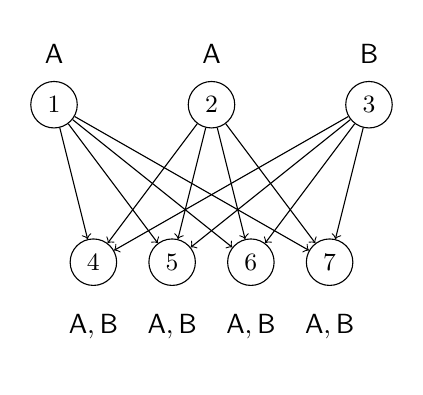
\begin{tikzpicture}
      \begin{scope}[every node/.style = {draw,circle}]
        \node[label=above:{$\sf A$}] (1) at (-2,0) {\small 1};
        \node[label=above:{$\sf A$}] (2) at ( 0,0) {\small 2};
        \node[label=above:{$\sf B$}] (3) at ( 2,0) {\small 3};
        \node[label=below:{$\sf A, B$}] (4) at (-1.5,-2) {\small 4};
        \node[label=below:{$\sf A, B$}] (5) at (-0.5,-2) {\small 5};
        \node[label=below:{$\sf A, B$}] (6) at ( 0.5,-2) {\small 6};
        \node[label=below:{$\sf A, B$}] (7) at ( 1.5,-2) {\small 7};
      \end{scope}
      \path[every edge/.style={draw,->}] {
        \foreach \x in {1,2,3} {
          \foreach \y in {4,5,6,7} {
            (\x) edge (\y)
          }
        }
      };
    \end{tikzpicture}
    \caption{Example interpretation $\mathcal{I}$ for
      \Cref{expl:nonredundant-implicational-base-yields-redundant-gci-base}.}
    \label{fig:example-interpretation-1}
  \end{figure}

  So let $N_C := \set{ \mathsf{A}, \mathsf{B} }$ and $N_R := \set{ \mathsf{r} }$.
  Consider the interpretation $\mathcal{I}$ as given in
  \Cref{fig:example-interpretation-1}, where every edge is labeled with $\mathsf{r}$.  Then
  \begin{align*}
    \conf_{\mathcal{I}}(\mathsf{A} \sqsubseteq \mathsf{B}) &= \frac 2 3\\
    \conf_{\mathcal{I}}(\mathsf{\exists r. A} \sqsubseteq \mathsf{\exists r. B}) &= 1,
  \end{align*}
  thus following our argumentation from above we can choose $c = \frac 1 2$, say.  Then we
  want to find a irredundant set $\mathcal{L}$ of implications such that $\mathcal{L} \cup
  \mathcal{S}_{\mathcal{I}}$ is a confident base of $\Th_c(\con K_{\mathcal{I}})$ and
  $\mathcal{L}$ contains both $\set{ \mathsf{A} } \to \set{ \mathsf{B} }$ and $\set{
    \mathsf{\exists r. A} } \to \set{ \mathsf{\exists r. (A \sqcap B)} }$.  We find
  \begin{multline*}
    M_{\mathcal{I}} = \{\, \sf \bot, A, B, \exists r.(A \sqcap \exists r.(A \sqcap B)), \\
    \sf \exists r.(B \sqcap \exists r.(A \sqcap B)), \exists r.(A \sqcap B), \exists
    r.\exists r.(A \sqcap B), \exists r.A, \exists r.B, \exists r.\top \,\},
  \end{multline*}
  and $\con K_{\mathcal{I}}$ is as shown in
  \Cref{fig:induced-formal-context-of-example-interpretation-1}.

  \begin{figure}[tp]
    \centering
    \newcommand{\attbox}[1]{\parbox[b][1ex][b]{1cm}{
        \rotatebox{45}{$\sf #1$}}}
    \vspace*{1.5cm}
    \begin{equation*}
      \begin{array}[c]{c||*{3}{c}*{7}{>{}c<{}}}
        \con{K}_{\mathcal{I}} & \bot & \sf A & \sf B &
        \hbox to 1cm{\attbox{\exists r.(A \sqcap \exists r.(A \sqcap B))}} &
        \attbox{\exists r.(B \sqcap \exists r.(A \sqcap B))} &
        \attbox{\exists r.(A \sqcap B)} &
        \attbox{\exists r.\exists r.(A \sqcap B)} &
        {\sf \exists r.A} &
        {\sf \exists r.B} &
        {\sf \exists r.\top} \\
        \hline
        1 & . & \times & . & . & . & \times & . & \times & \times & \times \\
        2 & . & \times & . & . & . & \times & . & \times & \times & \times \\
        3 & . & . & \times & . & . & \times & . & \times & \times & \times \\
        4 & . & \times & \times & . & . & . & . & . & . & . \\
        5 & . & \times & \times & . & . & . & . & . & . & . \\
        6 & . & \times & \times & . & . & . & . & . & . & . \\
        7 & . & \times & \times & . & . & . & . & . & . & . \\
      \end{array}
    \end{equation*}
    \caption{Induced formal context of $\mathcal{I}$ as in
      \Cref{expl:nonredundant-implicational-base-yields-redundant-gci-base}.}
    \label{fig:induced-formal-context-of-example-interpretation-1}
  \end{figure}

  By \Cref{thm:conf-base} the set $\Can(\con K_{\mathcal{I}}) \cup \Conf(\mathcal{I}, c)$
  is a confident base of $\Th_c(\con K_{\mathcal{I}})$.  An irredundant subset
  $\mathcal{L}$ of this base which is still a base of $\Th_c(\con K_{\mathcal{I}})$ with
  background knowledge $\mathcal{S}_{\mathcal{I}}$ is given by the following list of
  implications:
  \begin{align*}
    \emptyset &\to \set{\sf A},\\
    \set{\sf A}    &\to \set{\sf B},\\
    \set{\sf \exists r.A} &\to \set{\sf \exists r.(A \sqcap B)},\\
    \set{\sf \exists r.B} &\to \set{\sf \exists r.(A \sqcap B)},\\
    \set{\sf \exists r.\top} &\to \set{\exists r.(A \sqcap B)},\\
    \set{\sf A, B, \exists r.(A \sqcap B)} &\to \set{\bot},\\
    \set{\sf \exists r.\exists r.(A \sqcap B)} &\to \set{\bot},\\
    \set{\sf \exists r.(B \sqcap \exists r.(A \sqcap B))} &\to \set{\bot},\\
    \set{\sf \exists r.(A \sqcap \exists r.(A \sqcap B))} &\to \set{\bot}.
  \end{align*}
  Then $\mathcal{L}$ is irredundant and by
  \Cref{cor:using-background-knowledge-for-confident-bases} the set $\bigsqcap
  \mathcal{L}$ is a base of $\Th_c(\mathcal{I})$.  But $\bigsqcap \mathcal{L}$ contains
  the GCIs $\mathsf{A \sqsubseteq B}$ and $\mathsf{\exists r. A \sqsubseteq \exists r. (A
    \sqcap B)}$, and thus $\bigsqcap \mathcal{L}$ is not irredundant.
\end{Example}

Instead of only considering irredundant bases of $\Th_c(\con K_{\mathcal{I}})$, we can go
even a step further and consider \emph{minimal} bases of $\Th_c(\con K_{\mathcal{I}})$.
For this we recall that if $\mathcal{L}$ is a base of $\Th_c(\con K_{\mathcal{I}})$, then
the canonical base $\Can(\mathcal{L})$ of $\mathcal{L}$ is a minimal base of $\Th_c(\con
K_{\mathcal{I}})$.\footnote{Note that we have only introduced the canonical base for
  formal contexts, but by \Cref{prop:context-model-for-implications} we can represent
  every set $\mathcal{L}$ is a base of a formal context $\con K_{\mathcal{L}}$.  Then
  $\Can(\mathcal{L}) := \Can(\con K_{\mathcal{L}})$.  Note that this definition is
  independent from the context $\con K_{\mathcal{L}}$ we use.}  Since $\Cn(\mathcal{L}) =
\Cn(\Can(\mathcal{L}))$, we know that $\Can(\mathcal{L})$ is also a base of $\Th_c(\con
K_{\mathcal{I}})$.  In particular, if $\mathcal{L} = \Th_c(\con K_{\mathcal{I}})$ we can
consider $\Can(\Th_c(\con K_{\mathcal{I}}))$ as a minimal base of $\Th_c(\con
K_{\mathcal{I}})$.\footnote{Also note that $\Can(\mathcal{L}) = \Can(\Th_c(\con
  K_{\mathcal{I}}))$ for all bases $\mathcal{L}$ of $\Th_c(\con K_{\mathcal{I}})$.}  In
this case also we obtain that $\bigsqcap \Can(\Th_c(\con K_{\mathcal{I}}))$ is a finite
base of $\Th_c(\mathcal{I})$, as the following argumentation shows.

\begin{Corollary}
  \label{cor:bases-of-implications-to-bases-of-gcis}
  Let $\mathcal{I}$ be a finite interpretation, let $c \in [0,1]$ and let $\mathcal{K}
  \subseteq \Imp(M_{\mathcal{I}})$ be a base of $\Th_c(\con K_{\mathcal{I}})$.  Then
  $\bigsqcap \mathcal{K}$ is a base of $\Th_c(\mathcal{I})$.
\end{Corollary}
\begin{Proof}
  By \Cref{thm:confident-bases-of-GCIs-from-confident-bases-of-implications} we know that
  $\bigsqcap \Th_c(\con K_{\mathcal{I}})$ is a finite confident base of
  $\Th_c(\mathcal{I})$.  As $\mathcal{K}$ is a base of $\Th_c(\con K_{\mathcal{I}})$ we
  can infer from \Cref{lem:implicational-entailment-implies-gci-entailment} that
  $\bigsqcap \mathcal{K}$ is also complete for $\bigsqcap \Th_c(\con K_{\mathcal{I}})$.
  We thus obtain that $\bigsqcap \mathcal{K}$ is complete for $\Th_c(\mathcal{I})$.

  On the other hand, since $\mathcal{K}$ is a base of $\Th_c(\con K_{\mathcal{I}})$, it is
  also true that $\Th_c(\con K_{\mathcal{I}})$ is a base of $\mathcal{K}$.  But then all
  implications in $\mathcal{K}$ are entailed by $\Th_c(\con K_{\mathcal{I}})$, and
  \Cref{lem:implicational-entailment-implies-gci-entailment} yields that all GCIs in
  $\bigsqcap \mathcal{K}$ are entailed by $\bigsqcap \Th_c(\con K_{\mathcal{I}}) \subseteq
  \Th_c(\mathcal{I})$.  Thus, $\bigsqcap \mathcal{K}$ is also sound for
  $\Th_c(\mathcal{I})$, and in sum we obtain that $\bigsqcap \mathcal{K}$ is a finite base
  of $\Th_c(\mathcal{I})$.
\end{Proof}

The approach of considering the canonical base of $\Th_c(\con K)$ has the potential
drawback, however, that we cannot guarantee anymore that the base itself is a confident
base, \ie it could happen that $\bigsqcap \Can(\Th_c(\con K)) \subseteq
\Th_c(\mathcal{I})$ does not hold.

\subsection{Completing Sets of GCIs}
\label{sec:completing-sets-of-gcis}

The bases we have obtained in \Cref{cor:weakened-luxenburger-base-for-gcis} consisted of
two parts, namely a complete subset $\mathcal{B}$ of $\Lux(\mathcal{I}, c)$ and a set
$\mathcal{L}$ of valid GCIs such that $\mathcal{L} \cup \mathcal{B}$ is complete for
$\mathcal{I}$.  In this section we are going to show that we can, given the set
$\mathcal{B}$, compute the set $\mathcal{L}$ in such a way that $\mathcal{L} \cup
\mathcal{B}$ is complete for $\Th(\mathcal{I})$.  The results of this section have
previously been published in~\cite{Borchmann:confident-GCIs}.

The idea we want to exploit for this is borrowed from formal concept analysis: if
$\mathcal{B}$ is a set of implications, then we can find a set $\mathcal{L}$ of
implications valid in a formal context $\con K$ such that $\mathcal{L}$ has minimal
cardinality.  More precisely, the set
\begin{equation*}
  \mathcal{L} := \Can(\con K, \mathcal{B})
\end{equation*}
has this property by \Cref{thm:canonical-base-with-arbitrary-background-knowledge}.  What
we want to do in this section is to lift this result to the level of general concept
inclusions.

To this end, we need to transform sets of general concept inclusions into sets of
implications.  For this, we make use of \emph{projections} $\pr_M$ as introduced in
\Cref{sec:induced-contexts}.  More precisely, if $M$ is a set of concept descriptions and
$\mathcal{B}$ is a set of GCIs, then we define
\begin{equation*}
  \pr_M(\mathcal{B}) := \set{ \pr_M(C) \to \pr_M(D) \mid (C \sqsubseteq D) \in \mathcal{B} }.
\end{equation*}
For $M = M_{\mathcal{I}}$, we can take the set $\pr_{M_{\mathcal{I}}}(\mathcal{B})$ and
compute $\Can(\con K_{\mathcal{I}}, \pr_{M_{\mathcal{I}}}(\mathcal{B}))$.  It is then true
that the set
\begin{equation*}
  \mathcal{B} \cup \set{ \bigsqcap U \sqsubseteq (\bigsqcap U)^{\mathcal{I}\mathcal{I}} \mid (U \to U'')
    \in \Can(\con K_{\mathcal{I}}, \pr_{M_{\mathcal{I}}}(\mathcal{B})) }
\end{equation*}
is complete for $\mathcal{I}$, provided that the concept descriptions in $\mathcal{B}$ are
all expressible in terms of $M_{\mathcal{I}}$.

This result already appeared in \cite[Theorem~5.12]{Diss-Felix}, however only for the case
that $\mathcal{B}$ is empty.  We shall generalize this result to also cover the case that
$\mathcal{B}$ contains arbitrary GCIs.  The proof of this generalization is similar to the
one of \cite[Theorem~5.12]{Diss-Felix}.

\begin{Theorem}
  \label{thm:gci-completion-simple-version}
  Let $\mathcal{I}$ be a finite interpretation over $N_C$ and $N_R$, and let $\mathcal{B}$
  be a set of GCIs over $N_C$ and $N_R$, where all concept descriptions appearing in
  $\mathcal{B}$ are expressible in terms of $M_{\mathcal{I}}$.  Let $\mathcal{L} \subseteq
  \Th(\con K_{\mathcal{I}})$ such that
  \begin{enumerate}[i. ]
  \item\label{item:18} $\mathcal{L} \cup \pr_{M_{\mathcal{I}}}(\mathcal{B})$ is complete
    for $\con K_{\mathcal{I}}$, and
  \item\label{item:19} $\mathcal{L}$ only contains implications of the form $A \to A''$
    with $A \subseteq M_{\mathcal{I}}$.
  \end{enumerate}
  Then $\bigsqcap \mathcal{L} \cup \mathcal{B}$ is complete for $\mathcal{I}$.
\end{Theorem}
\begin{Proof}
  We show that for each $U \subseteq M_{\mathcal{I}}$ it is true that
  \begin{equation*}
    \bigsqcap \mathcal{L} \cup \mathcal{B} \models (\bigsqcap U \sqsubseteq (\bigsqcap
    U)^{\mathcal{I}\mathcal{I}}).
  \end{equation*}
  If we establish this fact, then \Cref{thm:Felix-base-B2} immediately yields that
  $\bigsqcap \mathcal{L} \cup \mathcal{B}$ is complete for $\Th(\mathcal{I})$.

  Let $\mathcal{J}$ be a finite interpretation such that $\mathcal{J} \models (\bigsqcap
  \mathcal{L} \cup \mathcal{B})$.  Let us write $\cdot^{\prime_{\mathcal{I}}}$ for the
  derivation operators in $\con K_{\mathcal{I}, M_{\mathcal{I}}}$, and
  $\cdot^{\prime_{\mathcal{J}}}$ for the derivation operators in $\con K_{\mathcal{J},
    M_{\mathcal{I}}}$.  We shall then show the following claims
  \begin{enumerate}[i. ]
  \item\label{item:20} $\con K_{\mathcal{J}, M_{\mathcal{I}}} \models (\mathcal{L} \cup
    \pr_{M_{\mathcal{I}}}(\mathcal{B}))$,
  \item $\con K_{\mathcal{J}, M_{\mathcal{I}}} \models (U \to
    U^{\prime_{\mathcal{I}}\prime_{\mathcal{I}}})$ for all $U \subseteq M_{\mathcal{I}}$,
    and finally
  \item $\mathcal{J} \models (\bigsqcap U \sqsubseteq (\bigsqcap
    U)^{\mathcal{I}\mathcal{I}})$ for all $U \subseteq M_{\mathcal{I}}$.
  \end{enumerate}

  To show the first claim we start with some preparations.  Let $U \subseteq
  M_{\mathcal{I}}$.  Then by \Cref{prop:connection-I-prime-2} it is true that
  \begin{equation}
    \label{eq:29}
    (\bigsqcap U)^{\mathcal{J}} = U^{\prime_{\mathcal{J}}}.
  \end{equation}
  Furthermore, the concept description $(\bigsqcap U)^{\mathcal{I}\mathcal{I}}$ is
  expressible in terms of $M_{\mathcal{I}}$ by
  \Cref{lem:mmsc-are-expressible-in-terms-of-M_I}.  From this we can infer with
  \Cref{lem:characterizing-expressible-in-terms-of} that
  \begin{equation*}
    (\bigsqcap U)^{\mathcal{I}\mathcal{I}} \equiv \bigsqcap
    \pr_{M_{\mathcal{I}}}((\bigsqcap U)^{\mathcal{I}\mathcal{I}}).
  \end{equation*}
  Then \Cref{cor:mmsc-lattice} yields
  \begin{equation}
    \label{eq:30}
    \begin{aligned}
      ((\bigsqcap U)^{\mathcal{I}\mathcal{I}})^{\mathcal{J}}
      &= (\bigsqcap \pr_{M_{\mathcal{I}}}((\bigsqcap
      U)^{\mathcal{I}\mathcal{I}}))^{\mathcal{J}} \\
      &= (\pr_{M_{\mathcal{I}}}((\bigsqcap
      U)^{\mathcal{I}\mathcal{I}}))^{\prime_{\mathcal{J}}} \\
      &= U^{\prime_{\mathcal{I}}\prime_{\mathcal{I}}\prime_{\mathcal{J}}}.
    \end{aligned}
  \end{equation}
  Now let $(U \to U^{\prime_{\mathcal{I}}\prime_{\mathcal{I}}}) \in \mathcal{L}$.  Then
  $\mathcal{J} \models (\bigsqcap U \sqsubseteq (\bigsqcap U)^{\mathcal{I}\mathcal{I}})$,
  and therefore
  \begin{equation*}
    (\bigsqcap U)^{\mathcal{J}} \subseteq ((\bigsqcap U)^{\mathcal{I}\mathcal{I}})^{\mathcal{J}},
  \end{equation*}
  and \Cref{eq:29} and (\Cref{eq:30}) yield
  \begin{equation*}
    U^{\prime_{\mathcal{J}}} \subseteq U^{\prime_{\mathcal{I}}\prime_{\mathcal{I}}\prime_{\mathcal{J}}},
  \end{equation*}
  \ie $\con K_{\mathcal{J}, M_{\mathcal{I}}} \models (U \to
  U^{\prime_{\mathcal{I}}\prime_{\mathcal{I}}})$.  Thus, $\con K_{\mathcal{J},
    M_{\mathcal{I}}} \models \mathcal{L}$.

  Let $(C \sqsubseteq D) \in \mathcal{B}$.  It remains to show that
  $\pr_{M_{\mathcal{I}}}(C) \to \pr_{M_{\mathcal{I}}}(D)$ holds in $\con K_{\mathcal{J},
    M_{\mathcal{I}}}$.  It is true that $\mathcal{J} \models (C \sqsubseteq D)$, \ie
  $C^{\mathcal{J}} \subseteq D^{\mathcal{J}}$.  Since both $C, D$ are expressible in terms
  of $M_{\mathcal{I}}$, \Cref{lem:characterizing-expressible-in-terms-of} yields
  \begin{equation*}
    (\bigsqcap \pr_{M_{\mathcal{I}}}(C))^{\mathcal{J}} \subseteq (\bigsqcap
    \pr_{M_{\mathcal{I}}}(D))^{\mathcal{J}}
  \end{equation*}
  and thus, using \Cref{eq:29} again,
  \begin{equation*}
    \pr_{M_{\mathcal{I}}}(C)^{\prime_{\mathcal{J}}} \subseteq \pr_{M_{\mathcal{I}}}(D)^{\prime_\mathcal{J}},
  \end{equation*}
  \ie $\con K_{\mathcal{J}, M_{\mathcal{I}}} \models (\pr_{M_{\mathcal{I}}}(C) \to
  \pr_{M_{\mathcal{I}}}(D))$.  Thus we have shown that $\con K_{\mathcal{J},
    M_{\mathcal{I}}} \models \mathcal{B}$.  This proves the first claim.

  Now let $U \subseteq M_{\mathcal{I}}$.  Then $\con K_{\mathcal{I}} \models (U \to
  U^{\prime_{\mathcal{I}}\prime_{\mathcal{I}}})$.  Since $\mathcal{L} \cup
  \pr_{M_{\mathcal{I}}}(\mathcal{B})$ is complete for $\con K_{\mathcal{I}}$, we obtain
  \begin{equation*}
    \mathcal{L} \cup \pr_{M_{\mathcal{I}}}(\mathcal{B}) \models (U \to
    U^{\prime_{\mathcal{I}}\prime_{\mathcal{I}}}).
  \end{equation*}
  Since $\con K_{\mathcal{J}, M_{\mathcal{I}}} \models \mathcal{L} \cup
  \pr_{M_{\mathcal{I}}}(\mathcal{B})$, it is true that
  \begin{equation*}
    \con K_{\mathcal{J}, M_{\mathcal{I}}} \models (U \to U^{\prime_{\mathcal{I}}\prime_{\mathcal{I}}}),
  \end{equation*}
  \ie $U^{\prime_{\mathcal{J}}} \subseteq
  U^{\prime_{\mathcal{I}}\prime_{\mathcal{I}}\prime_{\mathcal{J}}}$.  Using \Cref{eq:29}
  and \Cref{eq:30} again yields
  \begin{equation*}
    (\bigsqcap U)^{\mathcal{J}} \subseteq ((\bigsqcap U)^{\mathcal{I}\mathcal{I}})^{\mathcal{J}},
  \end{equation*}
  \ie $\mathcal{J} \models (\bigsqcap U \sqsubseteq (\bigsqcap
  U)^{\mathcal{I}\mathcal{I}})$.  Since $U \subseteq M_{\mathcal{I}}$ was chosen
  arbitrarily, we have thus shown that $\bigsqcap \mathcal{L} \cup \mathcal{B}$ is
  complete for $\mathcal{I}$.
\end{Proof}

We can apply this theorem to our setting of computing finite confident bases as follows.
Let $\mathcal{C} \subseteq \Lux(\mathcal{I}, c)$ be complete for $\Lux(\mathcal{I}, c)$.
If we compute $\mathcal{L} := \Can(\con K_{\mathcal{I}},
\pr_{M_{\mathcal{I}}}(\mathcal{B}))$, then $\mathcal{L}$ is as required by the above
theorem, and thus $\bigsqcap \mathcal{L} \cup \mathcal{B}$ is complete for $\mathcal{I}$.
By \Cref{cor:weakened-luxenburger-base-for-gcis} the set $\bigsqcap \mathcal{L} \cup
\mathcal{C}$ is a finite confident base of $\Th_c(\mathcal{I})$.

Of course, we can also include the implications in $\mathcal{S}_{\mathcal{I}}$ as
background knowledge when computing $\mathcal{L}$.  To see this we observe that the proof
of \Cref{thm:gci-completion-simple-version} still works if we include
$\mathcal{S}_{\mathcal{I}}$ in the computation of $\mathcal{L}$.  Then \cref{item:20} of
the proof would be extended to also claim that $\con K_{\mathcal{J}, M_{\mathcal{I}}}
\models \mathcal{S}_{\mathcal{I}}$, which is, however, true for all induced contexts with
attribute set $M_{\mathcal{I}}$.

\begin{Corollary}
  \label{cor:gci-completion-with-S_I}
  Let $\mathcal{I}$ be a finite interpretation over $N_C$ and $N_R$, and let $\mathcal{C}
  \subseteq \Lux(\mathcal{I}, c)$ be complete for $\Lux(\mathcal{I}, c)$.  Define
  \begin{equation*}
    \mathcal{L} := \Can(\con K_{\mathcal{I}}, \pr_{M_{\mathcal{I}}}(\mathcal{C}) \cup \mathcal{S}_{\mathcal{I}}).
  \end{equation*}
  Then $\bigsqcap \mathcal{L} \cup \mathcal{C}$ is a finite confident base of
  $\Th_c(\mathcal{I})$.
\end{Corollary}

For $c = 0$ we obtain $\Lux(\mathcal{I}, c) = \emptyset$, and thus we are back in the case
of valid GCIs.  For this we know from \Cref{thm:Felix-5.18} that the set $\bigsqcap
\mathcal{L}$ in the previous corollary is \emph{minimal} with respect to being a base of
$\mathcal{I}$.  A natural question is now to ask whether we can also expect such a
minimality result to be true in the case of GCIs with high confidence, \ie whether
$\bigsqcap \mathcal{L}$ is minimal with respect to $\bigsqcap \mathcal{L} \cup
\mathcal{B}$ being a finite confident base of $\Th_c(\mathcal{I})$.  The next example
shows that this is not the case.

\begin{Example}
  \label{expl:no-minimality}
  Let $N_C = \set{ \mathsf{A}, \mathsf{B} }$ and $N_R = \set{ \mathsf{r} }$ and consider
  the finite interpretation $\mathcal{I} = (\Delta^{\mathcal{I}}, \cdot^{\mathcal{I}})$ as
  given in \Cref{fig:no-minimality}.

  \begin{figure}[tp]
    \centering
    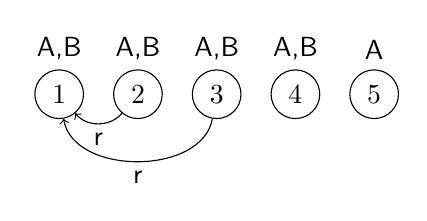
\begin{tikzpicture}
      \node[draw, circle, label=above:{\textsf{A,B}}] (1) at (0,0) {1};
      \node[draw, circle, label=above:{\textsf{A,B}}] (2) at (1,0) {2};
      \node[draw, circle, label=above:{\textsf{A,B}}] (3) at (2,0) {3};
      \node[draw, circle, label=above:{\textsf{A,B}}] (4) at (3,0) {4};
      \node[draw, circle, label=above:{\textsf{A}}] (5) at (4,0) {5};
      \draw[->] (2) edge[bend left=50] node[midway,below] {\textsf{r}} (1);
      \draw[->] (3) edge[bend left=80] node[midway,below] {\textsf{r}} (1);
    \end{tikzpicture}
    \caption{Interpretation for \Cref{expl:no-minimality}}
    \label{fig:no-minimality}
  \end{figure}

  If $X \subseteq \Delta^{\mathcal{I}}$ is such that $5 \in X$, then $X^{\mathcal{I}} =
  \mathsf{A}$.  If $5 \notin X$ but $1 \in X$ or $4 \in X$, then $X^{\mathcal{I}} =
  \mathsf{A} \sqcap \mathsf{B}$.  Otherwise, $X^{\mathcal{I}} = \mathsf{A \sqcap B \sqcap
    \exists r. A \sqcap B}$.  Thus the set of model-based most-specific concept
  descriptions of $\mathcal{I}$ up to equivalence is
  \begin{equation*}
    \set{ \bot, \mathsf{A}, \mathsf{A \sqcap B}, \mathsf{A \sqcap B \sqcap \exists
        r.(A \sqcap B)} }
  \end{equation*}
  and thus we obtain
  \begin{equation*}
    M_{\mathcal{I}} := \set{ \bot, \mathsf{A}, \mathsf{B}, \mathsf{\exists r. A},
      \mathsf{\exists r. (A \sqcap B)}, \mathsf{\exists r. (A \sqcap B \sqcap \exists
        r. (A \sqcap B))} }.
  \end{equation*}
  The induced context is shown in \Cref{fig:no-minimality-induced-context}.

  \begin{figure}[tp]
    \centering
    \begin{math}
      \begin{array}{c|*{6}{c}}
        \toprule
        ~ & \bot & \mathsf{A} & \mathsf{B} & \mathsf{\exists r. A} & \mathsf{\exists r. (A
          \sqcap B)} & \mathsf{\exists r. (A \sqcap B \sqcap \exists r. (A \sqcap B))} \\
        \midrule
        1 & & \times & \times \\
        2 & & \times & \times & \times & \times \\
        3 & & \times & \times & \times & \times \\
        4 & & \times & \times \\
        5 & & \times  \\
        \bottomrule
      \end{array}
    \end{math}
    \caption{Induced Context of \Cref{fig:no-minimality}}
    \label{fig:no-minimality-induced-context}
  \end{figure}

  Let $c = \frac 4 5$.  Then $\Conf(\con K_{\mathcal{I}}, c) = \set{ \set{ \mathsf{A} }
    \to \set{ \mathsf{A}, \mathsf{B} } }$, thus
  \begin{equation*}
    \Conf(\mathcal{I}, c) = \set{ \mathsf{A} \sqsubseteq \mathsf{A \sqcap B} }.
  \end{equation*}
  Set $\mathcal{B} := \Conf(\mathcal{I}, c)$.  Then $\pr_{M_{\mathcal{I}}}(\mathcal{B}) =
  \Conf(\con K_{\mathcal{I}}, c)$.  Let
  \begin{equation*}
    U := \set{ \mathsf{\exists r. A}, \mathsf{A}, \mathsf{B} }.
  \end{equation*}
  The $U$ is closed under $\mathcal{S}_{\mathcal{I}}$.  Furthermore, $U$ is a
  $\pr_{M_{\mathcal{I}}}(\mathcal{B})$-pseudo-intent of $\con K_{\mathcal{I}}$:
  $\emptyset$ is a $\pr_{M_{\mathcal{I}}}(\mathcal{B})$-pseudo-intent of $\con
  K_{\mathcal{I}}$, and $\emptyset'' = \set{ \mathsf{A} } \subseteq U$.  The set $\set{
    \mathsf{A} }$ is an intent of $\con K_{\mathcal{I}}$, and the sets $\set{ \mathsf{B}
  }$ and $\set{ \mathsf{\exists r. A} }$ are not supersets of $\emptyset'' = \set{
    \mathsf{A} }$.  The set $\set{ \mathsf{A}, \mathsf{B} }$ is again an intent of $\con
  K_{\mathcal{I}}$, $\set{ \mathsf{\exists r. A}, \mathsf{A} }$ is not closed under
  $\pr_{M_{\mathcal{I}}}(\mathcal{B})$ and $\set{ \mathsf{\exists r. A}, \mathsf{B} }$
  does not contain $A$.  Thus, the only $\pr_{M_{\mathcal{I}}}(\mathcal{B})$-pseudo-intent
  of $\con K_{\mathcal{I}}$ contained in $U$ is $\emptyset$, and its closure is again
  contained in $U$.  Thus, $U$ is a $\pr_{M_{\mathcal{I}}}(\mathcal{B})$-pseudo-intent of
  $\con K_{\mathcal{I}}$.

  Therefore, $(U \to U'') \in \Can(\con K_{\mathcal{I}},
  \pr_{M_{\mathcal{I}}}(\mathcal{B}) \cup \mathcal{S}_{\mathcal{I}})$, \ie
  \begin{equation*}
    (\set{ \mathsf{\exists r. A}, \mathsf{A}, \mathsf{B} } \to \set{ \mathsf{\exists r. (A
        \sqcap B)} }) \in \Can(\con K_{\mathcal{I}}, \pr_{M_{\mathcal{I}}}(\mathcal{B}) \cup
    \mathcal{S}_{\mathcal{I}}).
  \end{equation*}
  This yields that
  \begin{equation*}
    (\mathsf{\exists r. A \sqcap A \sqcap B} \sqsubseteq \mathsf{\exists r. (A \sqcap B)})
    \in \bigsqcap \Can(\con K_{\mathcal{I}}, \pr_{M_{\mathcal{I}}}(\mathcal{B}) \cup \mathcal{S}_{\mathcal{I}}).
  \end{equation*}
  But this GCI is entailed by $\mathcal{B}$, so the set $\bigsqcap \Can(\con
  K_{\mathcal{I}}, \pr_{M_{\mathcal{I}}}(\mathcal{B}) \cup \mathcal{S}_{\mathcal{I}}) \cup
  \mathcal{B}$ is not irredundant.  In particular, $\bigsqcap \Can(\con K_{\mathcal{I}},
  \pr_{M_{\mathcal{I}}}(\mathcal{B}) \cup \mathcal{S}_{\mathcal{I}})$ is not minimal with
  respect to the property that it forms together with $\mathcal{B}$ a confident base of
  $\Th_c(\mathcal{I})$.
\end{Example}

The main reason why the minimality statement fails is that entailment between GCIs can
happen ``behind the quantifier'': if $\mathcal{B} = \set{ \mathsf{A} \sqsubseteq
  \mathsf{B} }$, then $\mathcal{B}$ entails $\mathsf{\exists r. A} \sqsubseteq
\mathsf{\exists r. B}$.  This entailment process can usually not be simulated by
implications, as they are not allowed to consider the structure of the attributes in a
formal context.

It is possible to find a special case where entailment behind the quantifier cannot
happen: if $\mathcal{B}$ is a set of \emph{valid} GCIs of $\mathcal{I}$ and if $C =
\bigsqcap U$ for $U \subseteq M_{\mathcal{I}}$ and $U \neq \emptyset$.  In this case, $C$
can be written as
\begin{equation*}
  C = \bigsqcap V \sqcap \bigsqcap_{(r, Z) \in \Pi} \exists r. Z^{\mathcal{I}}
\end{equation*}
for some $V \subseteq N_C$ and some $\Pi \subseteq N_R \times
\subsets{\Delta^{\mathcal{I}}}$.  Then one can argue that the concept descriptions
$Z^{\mathcal{I}}$ behind the quantifier are already ``closed under entailment'' with
respect to $\mathcal{B}$, because they are model-based most-specific concept descriptions
and all GCIs in $\mathcal{B}$ are valid in $\mathcal{I}$.  Thus, if a GCI $C \sqsubseteq
D$ is entailed by $\mathcal{B}$, it must happen on the top-level of the concept
descriptions, and this entailment can then be simulated by implications.

A formal argumentation requires the notions of \emph{simulations} between \EL description
graphs, which have not introduced in this work.  For more details on this we refer to
Lemma~5.16 and the proof of Theorem~5.18 in~\cite{Diss-Felix}.

\subsection{Unravelling \ELgfpbot Bases into \ELbot Bases}
\label{sec:unrav-elgfpb-bases}

So far we have only considered finite bases of $\Th_c(\mathcal{I})$ which consist of
\ELgfpbot concept descriptions.  As we had argued before, those concept descriptions may
actually be hard to read, over for those trained in logic.  Therefore, it would be
desirable to obtain bases which contain \ELbot concept descriptions only, as these are
potentially much easier to read.  To show that this is indeed possible is the purpose of
this section.  The argumentation we want to employ is again similar to the one used by
Distel; see \Cref{sec:base-all-valid}.

As a first step, as already discussed in \Cref{sec:base-all-valid}, we define an auxiliary
set $\mathcal{X}_{\mathcal{I}}$ that only contains \ELbot concept descriptions but
``captures'' entailment between \ELgfpbot concept descriptions.  For this, recall that
\Cref{lem:Felix-lemma-5.5} states that for a finite interpretation $\mathcal{I}$ and all
\ELgfpbot concept descriptions $C = (A, \mathcal{T})$ it is true that
\begin{equation*}
  C^{\mathcal{I}} = (C_d)^{\mathcal{I}},
\end{equation*}
where $d = \abs{ \Delta^{\mathcal{I}} } \cdot \abs{ N_D(\mathcal{T}) } + 1$.  Note that
the constant $d$ depends on the concept description $C$.  The set
$\mathcal{X}_{\mathcal{I}}$ is now defined as
\begin{equation*}
  \mathcal{X}_{\mathcal{I}} := \set{ (X^{\mathcal{I}})_d \sqsubseteq
    (X^{\mathcal{I}})_{d+1} \mid X \subseteq \Delta^{\mathcal{I}}, X \neq \emptyset }.
\end{equation*}
Note that $\mathcal{X}_{\mathcal{I}}$ is a set of valid GCIs of $\mathcal{I}$, and that
for each $X \subseteq \Delta^{\mathcal{I}}, X \neq \emptyset$ it is true that
\begin{equation*}
  ((X^{\mathcal{I}})_d)^{\mathcal{I}} = X^{\mathcal{I}\mathcal{I}} = ((X^{\mathcal{I}})_{d+1})^{\mathcal{I}}.
\end{equation*}

As already sketched in \Cref{sec:base-all-valid} the following claims hold.

\begin{Lemma}
  \label{lem:X_I-properties}
  Let $\mathcal{I}$ be a finite interpretation, let $Y \subseteq \Delta^{\mathcal{I}}$ and
  let $d \in \NN_0$ for $Y^{\mathcal{I}}$ as in \Cref{lem:Felix-lemma-5.5}.  Then
  \begin{enumerate}[i. ]
  \item $\mathcal{X}_{\mathcal{I}} \models ((Y^{\mathcal{I}})_k \sqsubseteq
    (Y^{\mathcal{I}})_{k+1})$ is true for all $k \geq d$, and
  \item $\mathcal{X}_{\mathcal{I}} \models ((Y^{\mathcal{I}})_d \sqsubseteq Y^{\mathcal{I}})$.
  \end{enumerate}
\end{Lemma}
\begin{Proof}
  For the first claim we observe that if $Y = \emptyset$, that then $Y^{\mathcal{I}} =
  \bot$ and nothing remains to be shown.  Therefore, let $Y \neq \emptyset$.  We shall
  show the claim by induction over $k$.

  For $k = d$ the claim is trivial, as $((Y^{\mathcal{I}})_d \sqsubseteq
  (Y^{\mathcal{I}})_{d+1}) \in \mathcal{X}_{\mathcal{I}}$.  For the step-case assume that
  \begin{equation}
    \label{eq:34}
    \mathcal{X}_{\mathcal{I}} \models ((Z^{\mathcal{I}})_{k-1} \sqsubseteq (Z^{\mathcal{I}})_k)
  \end{equation}
  is true for all $Z \subseteq \Delta^{\mathcal{I}}$.  Since $Y^{\mathcal{I}}$ is
  expressible in terms of $M_{\mathcal{I}}$, and $Y \neq \emptyset$, there exists $U
  \subseteq N_C$ and $\Pi \subseteq N_R \times \subsets{\Delta^{\mathcal{I}}}$ such that
  \begin{equation*}
    Y^{\mathcal{I}} \equiv \bigsqcap U \sqcap \bigsqcap_{(r, Z) \in \Pi} \exists r. Z^{\mathcal{I}}.
  \end{equation*}
  From \Cref{lem:unravelling-is-homomorphism} we obtain
  \begin{equation*}
    (Y^{\mathcal{I}})_k \equiv \bigsqcap U \sqcap \bigsqcap_{(r, Z) \in \Pi} \exists r.(Z^{\mathcal{I}})_{k-1}.
  \end{equation*}
  By the induction hypothesis \Cref{eq:34} we obtain that
  \begin{align*}
    (Y^{\mathcal{I}})_k
    &\sqsubseteq \bigsqcap U \sqcap \bigsqcap_{(r, Z) \in \Pi} \exists
    r. (Z^{\mathcal{I}})_k\\
    &\equiv (\bigsqcap U \sqcap \bigsqcap_{(r, Z) \in \Pi} \exists
    r. Z^{\mathcal{I}})_{k+1} \\
    &\equiv (Y^{\mathcal{I}})_{k+1}
  \end{align*}
  again using \Cref{lem:unravelling-is-homomorphism}.  This complete the induction step
  and the first claim is shown.

  We now show the second claim, namely
  \begin{equation*}
    \mathcal{X}_{\mathcal{I}} \models ((Y^{\mathcal{I}})_d \sqsubseteq Y^{\mathcal{I}})
  \end{equation*}
  for $Y \subseteq \Delta^{\mathcal{I}}$.  The case $Y = \emptyset$ is again trivial, so
  let $Y \neq \emptyset$.  Let $\mathcal{J}$ be a finite interpretation such that
  $\mathcal{J} \models \mathcal{X}_{\mathcal{I}}$.  Then the first claim yields
  \begin{equation*}
    ((Y^{\mathcal{I}})_d)^{\mathcal{J}} \subseteq ((Y^{\mathcal{I}})_{d+1})^{\mathcal{J}}
    \subseteq ((Y^{\mathcal{I}})_{d+2})^{\mathcal{J}} \subseteq \dots
  \end{equation*}
  From \Cref{lem:Felix-lemma-5.5} we obtain the existence of some $\ell \in \NN_0$ such
  that $((Y^{\mathcal{I}})_\ell)^{\mathcal{J}} = (Y^{\mathcal{I}})^{\mathcal{J}}$ is true.
  Therefore, $((Y^{\mathcal{I}})_d)^{\mathcal{J}} \subseteq
  (Y^{\mathcal{I}})^{\mathcal{J}}$ and thus $\mathcal{J} \models ((Y^{\mathcal{I}})_d
  \sqsubseteq Y^{\mathcal{I}})$.  Since \ELbot has the finite-model property, we obtain
  $\mathcal{X}_{\mathcal{I}} \models ((Y^{\mathcal{I}})_d \sqsubseteq Y^{\mathcal{I}})$ as
  required.
\end{Proof}

Now let $\mathcal{D}$ be a confident base of $\Th_c(\mathcal{I})$.  We then can partition
$\mathcal{D} = \mathcal{B} \cup \mathcal{C}$ such that $\mathcal{B} \subseteq
\Th(\mathcal{I})$ and $\mathcal{C} \cap \Th(\mathcal{I})$, \ie $\mathcal{B}$ contains all
valid GCIs of $\mathcal{D}$, and $\mathcal{C}$ contains everything else.  Without loss of
generality we can assume that $\mathcal{B}$ contains only GCIs of the form $E \sqsubseteq
E^{\mathcal{I}\mathcal{I}}$.  To construct an \ELbot base out of $\mathcal{D}$ we can now
proceed as described in the following theorem.

\begin{Theorem}
  \label{thm:unravelling-confident-bases}
  Let $\mathcal{I}$ be a finite interpretation, let $c \in [0,1]$ and let $\mathcal{D} =
  \mathcal{B} \cup \mathcal{C}$ be a finite confident base of $\Th_c(\mathcal{I})$, such
  that $\mathcal{B} \subseteq \Th(\mathcal{I})$, $\mathcal{C} \cap \Th(\mathcal{I}) \neq
  \emptyset$ and $\mathcal{B}$ contains only GCIs of the form $E \sqsubseteq
  E^{\mathcal{I}\mathcal{I}}$. Define
  \begin{align*}
    \mathcal{B}' &:= \set{ E_d \sqsubseteq (E^{\mathcal{I}\mathcal{I}})_d \mid (E
      \sqsubseteq E^{\mathcal{I}\mathcal{I}}) \in \mathcal{B} } \cup \set{ C_d \sqsubseteq
      (C^{\mathcal{I}\mathcal{I}})_d \mid (C \sqsubseteq D) \in \mathcal{C} },\\
    \mathcal{C}' &:= \set{ (C^{\mathcal{I}\mathcal{I}})_d \sqsubseteq
      (D^{\mathcal{I}\mathcal{I}})_d \mid (C \sqsubseteq D) \in \mathcal{C} }.
  \end{align*}
  Then the following statements hold:
  \begin{enumerate}[i. ]
  \item $\mathcal{C}' \subseteq \Th_c(\mathcal{I})$ and $\mathcal{B}' \cup \mathcal{C}'
    \cup \mathcal{X}_{\mathcal{I}} \models \mathcal{C}$.
  \item $\mathcal{B}' \cup \mathcal{C}' \cup \mathcal{X}_{\mathcal{I}} \models
    \mathcal{B}$.
  \end{enumerate}
  In particular, $\mathcal{B}' \cup \mathcal{C}' \cup \mathcal{X}_{\mathcal{I}}$ is a
  finite confident \ELbot base of $\Th_c(\mathcal{I})$.
\end{Theorem}

Note that $\mathcal{B}' \cup \mathcal{C}' \cup \mathcal{X}_{\mathcal{I}}$ only contains
\ELbot concept descriptions, and that all GCIs in $\mathcal{B}' \cup
\mathcal{X}_{\mathcal{I}}$ are valid in $\mathcal{I}$.

\begin{Proof}
  To see $\mathcal{C}' \subseteq \Th_c(\mathcal{I})$ recall that $(C_d)^{\mathcal{I}} =
  C^{\mathcal{I}}$ is true for each \ELgfpbot concept description $C$.  Thus, for $(C
  \sqsubseteq D) \in \mathcal{C}$ with $\abs{ C^{\mathcal{I}} } \neq \emptyset$ we obtain
  \begin{align*}
    \conf_{\mathcal{I}}( C \sqsubseteq D )
    &= \conf_{\mathcal{I}}( C^{\mathcal{I}\mathcal{I}} \sqsubseteq D^{\mathcal{I}\mathcal{I}} )\\
    &= \frac{ | ( C^{\mathcal{I}\mathcal{I}} \sqcap D^{\mathcal{I}\mathcal{I}}
      )^{\mathcal{I}} | }{ | C^{\mathcal{I}\mathcal{I}\mathcal{I}} | }\\
    &= \frac{ | (( C^{\mathcal{I}\mathcal{I}} \sqcap D^{\mathcal{I}\mathcal{I}}
      )_d)^{\mathcal{I}} | }{ | ((C^{\mathcal{I}\mathcal{I}})_d)^{\mathcal{I}} | }\\
    &= \frac{ | ( (C^{\mathcal{I}\mathcal{I}})_d \sqcap (D^{\mathcal{I}\mathcal{I}})_d
      )^{\mathcal{I}} | }{ | ((C^{\mathcal{I}\mathcal{I}})_d)^{\mathcal{I}} | }\\
    &= \conf_{\mathcal{I}}( (C^{\mathcal{I}\mathcal{I}})_d \sqsubseteq (D^{\mathcal{I}\mathcal{I}})_d )
  \end{align*}
  using \Cref{lem:unravelling-is-homomorphism}.  Clearly, if $C^{\mathcal{I}} =
  \emptyset$, then $(C_d)^{\mathcal{I}} = \emptyset$ and thus
  \begin{equation*}
    \conf_{\mathcal{I}}( C \sqsubseteq D ) = 1 = \conf_{\mathcal{I}}(
    (C^{\mathcal{I}\mathcal{I}})_d \sqsubseteq (D^{\mathcal{I}\mathcal{I}})_d ).
  \end{equation*}
  Since $\mathcal{C} \subseteq \Th_c(\mathcal{I})$, we therefore obtain $\mathcal{C}'
  \subseteq \Th_c(\mathcal{I})$ as required.

  We now show that $\mathcal{B}' \cup \mathcal{C}' \cup \mathcal{X}_{\mathcal{I}} \models
  \mathcal{C}$.  For this let $(C \sqsubseteq D) \in \mathcal{C}$.  Then we have
  \begin{align*}
    \emptyset &\models (C \sqsubseteq C_d)\\
    \mathcal{B}' &\models (C_d \sqsubseteq (C^{\mathcal{I}\mathcal{I}})_d)\\
    \mathcal{C}' &\models ((C^{\mathcal{I}\mathcal{I}})_d \sqsubseteq
    (D^{\mathcal{I}\mathcal{I}})_d)\\
    \mathcal{X}_{\mathcal{I}} &\models ((D^{\mathcal{I}\mathcal{I}})_d \sqsubseteq
    D^{\mathcal{I}\mathcal{I}})\\
    \emptyset &\models (D^{\mathcal{I}\mathcal{I}} \sqsubseteq D)
  \end{align*}
  using \Cref{lem:X_I-properties} for the second to last statement.  Therefore
  $\mathcal{B}' \cup \mathcal{C}' \cup \mathcal{X}_{\mathcal{I}} \models (C \sqsubseteq
  D)$ as required.

  We consider the second claim, namely that $\mathcal{B}' \cup \mathcal{C}' \cup
  \mathcal{X}_{\mathcal{I}} \models \mathcal{B}$.  To this end, let $(E \sqsubseteq
  E^{\mathcal{I}\mathcal{I}}) \in \mathcal{B}$.  Then
  \begin{align*}
    \emptyset &\models (E \sqsubseteq E_d)\\
    \mathcal{B}' &\models (E_d \sqsubseteq (E^{\mathcal{I}\mathcal{I}})_d)\\
    \mathcal{X}_{\mathcal{I}} &\models ((E^{\mathcal{I}\mathcal{I}})_d \sqsubseteq E^{\mathcal{I}\mathcal{I}})
  \end{align*}
  using \Cref{lem:X_I-properties} for the last statement.  Therefore,
  \begin{equation*}
    \mathcal{B}' \cup \mathcal{C}' \cup \mathcal{X}_{\mathcal{I}} \models (E \sqsubseteq
    E^{\mathcal{I}\mathcal{I}})
  \end{equation*}
  as required.
\end{Proof}

A drawback of this construction is that the set $\mathcal{X}_{\mathcal{I}}$ can be
exponentially large in the size of $\Delta^{\mathcal{I}}$, and so can be the \ELbot base
as described above.  Therefore, even if the original base $\mathcal{D}$ was small, the
described unravelling can transfer it into a much larger base.  It is not known to the
author whether this blowup is intrinsic to the task of transferring \ELgfpbot bases into
\ELbot bases, or whether it can be avoided by a different approach.

\section{GCIs with High Confidence from DBpedia}
\label{sec:exper-with-conf}

We have started this chapter by evaluating Distel's results in a practical scenario.
During this evaluation we have found out that the presence of errors in the data can
inhibit the usefulness of the results obtained by Distel's approach, and from this we have
motivated our study of GCIs with high confidence.  In this section, we want to apply our
findings about finite confident bases of $\Th_c(\mathcal{I})$ to the interpretation
$\Idbpedia$ we used before, and we want to see in how far the problem of errors in
$\Idbpedia$ can be alleviated by using GCIs with high confidence.

Let us assume that an ontology engineer wants to use the approach of considering GCIs with
high confidence to extract GCIs from some finite interpretation $\mathcal{I}$.  Then what
she has to do is that she needs to consider GCIs in $\Lux(\mathcal{I}, c)$ for a suitable
choice of $c$ and has to decide whether these GCIs should be added to the knowledge base.
To make this a practical approach, the set $\Lux(\mathcal{I}, c)$ should not be too large,
and the GCIs contained in there should not be incomprehensible.

We want to examine how this approach behaves for our data set $\Idbpedia$.  To this end,
we want to conduct several experiments, namely
\begin{enumerate}[i. ]
\item We want to examine the set $\Lux(\Idbpedia, 0.95)$ in detail, \ie we want to show
  how large these sets are and which GCIs are contained in them.  Moreover, we shall
  discuss how the ontology engineer proceeds in deciding whether the GCIs contained in
  these sets are true or not.
\item We want to compare the sizes of the sets $\Conf(\Idbpedia, c)$ and $\Lux(\Idbpedia,
  c)$ to see in how far we can remove redundancies from $\Conf(\Idbpedia, c)$ by using
  $\Lux(\Idbpedia, c)$ instead.  To this end, we shall compute for all $c \in \set{ 0.0,
    0.01, \dots, 0.99}$ the size of the sets $\Conf(\Idbpedia, c)$ and $\Lux(\Idbpedia,
  c)$ to see how the cardinality of these sets behaves.
\item Finally, we want to consider the size of the canonical base of $\Th_c(\con
  K_\Idbpedia)$ for $c \in \set{ 0.0, 0.01, \dots, 0.99 }$ to see how large this set can
  be.  Recall that $\bigsqcap \Can(\Th_c(\con K_\Idbpedia))$ is a finite base of
  $\Th_c(\mathcal{I})$, and the number of GCIs in this base can be considered as a
  ``small'' upper limit how many GCIs are needed to represent $\Th_c(\mathcal{I})$.
  Intuitively, if we decrease the value for $c$, we would expect that the number of GCIs
  contained in the canonical base decreases as well.  We shall see how far this is true
  for $\Idbpedia$.
\end{enumerate}

The experimental results presented in this section have been published previously in
\cite{Borchmann-LTCS-12-06}.

\subsection{Computing Confident Bases of $\Th_c(\Idbpedia)$ for $c = 0.95$}
\label{sec:comp-conf-bases}

Recall that we had constructed $\Idbpedia$ from the DBpedia data set by extracting all
individuals that are in a \textsf{child}-relationship in DBpedia, either as parent or as
child.  Since Wikipedia (from which DBpedia extracts its data) only contains articles
about (more or less) famous persons, we can thus consider $\Idbpedia$ as an interpretation
that contains all properties about the child-relations between \emph{famous} persons.  In
particular, if an element of $\Idbpedia$ does not have a \textsf{child}-successor in
$\Idbpedia$ (and this is not an error), then this does not necessarily mean that the
corresponding person does or did not have children -- it only means that the children were
not famous enough to deserve their own Wikipedia articles.

In the following we want to examine which GCIs we have to consider in addition to the base
$\mathcal{B}_{\Idbpedia}$ of $\Idbpedia$ we had computed in
\Cref{sec:computing-bases-from} if we want to consider also GCIs which have a high
confidence in $\Idbpedia$.  To this end, we shall compute the set $\Conf(\Idbpedia, c)$
for $c = 0.95$.  For this set we shall argue whether the GCIs contained in them can be
seen as being true in the domain which is represented by $\Idbpedia$.

Let $c = 0.95$.  We then can compute $\Conf(\Idbpedia, c)$ to be
\begin{align*}
  \{\,
  & \mathsf{\exists child. \top} \sqsubseteq \mathsf{Person}, \\
  & \mathsf{Place} \sqsubseteq \mathsf{PopulatedPlace},\\
  & \mathsf{\exists child. \exists child. \top} \sqcap \mathsf{\exists
    child. OfficeHolder} \\
  & \quad \sqsubseteq \mathsf{\exists child. (OfficeHolder \sqcap \exists child. \top)}
  \,\}
\end{align*}
Note that the actual GCIs computed are much more complex, since all concept descriptions
contained in $\Conf(\Idbpedia, c)$ actually have to be model-based most-specific concept
descriptions.  For readability, we have removed parts of the concept descriptions which
are already entailed by the base $\mathcal{B}_\Idbpedia$, so that the GCIs thus obtained
are still equivalent to the original ones.  Also notice that $\Lux(\Idbpedia, c) =
\Conf(\Idbpedia, c)$.

The first observation is that $\Lux(\Idbpedia, c)$ is small compared to the size of
$\mathcal{B}_\Idbpedia$, which has 1252 elements.  Thus, our potential ontology engineer
only has to consider three more GCIs.  Moreover, as we shall see later, accepting some of
the above GCIs may even lead to other GCIs in $\mathcal{B}_\Idbpedia$ to become
dispensable, and thus she does not have to consider those separately.

Let us now consider these three GCIs in detail.  The first one we had already seen in
\Cref{sec:computing-bases-from}, and there we had argued that this is actually true, since
the 4 counterexamples contained in $\Idbpedia$ were only due to errors.

The GCI $\mathsf{Place} \sqsubseteq \mathsf{PopulatedPlace}$ also sounds convincing: note
that places appear in $\Idbpedia$ only due to the fact that they are collected from
Wikipedia Infoboxes of articles which contain an entry for children, \ie which are
persons.  Since these places occur in the child-entries of infoboxes, they likely name the
places of birth of the corresponding children, and those places are usually populated.
Indeed, the only counterexamples for $\mathsf{Place \sqsubseteq PopulatedPlace}$ is
\textsf{Greenwich\_Village}, representing the corresponding district of Manhattan, New
York, which is certainly populated.  Thus also this counterexample is erroneous and we
accept the GCI as being true (in the domain represented by $\Idbpedia$).

On the other hand, the last GCI
\begin{equation*}
  \mathsf{\exists child. \exists child. \top \sqcap \exists child. OfficeHolder
    \sqsubseteq \exists child. ( OfficeHolder \sqcap \exists child. \top ) }
\end{equation*}
looks too specific.  The only counterexample contained in $\Idbpedia$ is the element
\begin{quote}
  \textsf{Pierre\_Samuel\_du\_Pont\_de\_Nemours}
\end{quote}
representing the french government official Pierre Samuel du Pont de Nemours.  He had two
sons, namely Victor Marie du Pont and Eleuthère Irénée du Pont.  The former became a
french diplomat and is therefore listed as \textsf{OfficeHolder} in $\Idbpedia$.  Although
he had four children, none of them were famous enough to receive their own Wikipedia
articles.  On the other hand, Eleuthère Irénée du Pont became a famous american industrial
(founder of the \emph{DuPont} company) and had several famous children which are all
listed in $\Idbpedia$.  Thus, given our understanding of the \textsf{child}-relation in
$\Idbpedia$ we can accept this counterexample as being valid, and we therefore reject this
GCI.

We have accepted the GCIs
\begin{equation*}
  \mathcal{B} := \set{ \mathsf{\exists child. \top \sqsubseteq Person},
    \mathsf{Place \sqsubseteq PopulatedPlace} }
\end{equation*}
as being valid although $\Idbpedia$ contains counterexamples for it.  It would now be
interesting to know what happened if we would include those two GCIs in a computation of a
base of $\Idbpedia$.  For this note that
\begin{equation*}
  \pr_{M_{\Idbpedia}}(\mathcal{B}) = \set{ \set{ \mathsf{\exists child. \top} } \to \set{
      \mathsf{Person} }, \set{ \mathsf{Place} } \to \set{ \mathsf{PopulatedPlace} } }.
\end{equation*}
If we now compute
\begin{equation*}
  \mathcal{L} := \Can(\con K_\Idbpedia, \pr_{M_{\Idbpedia}}(\mathcal{B}) \cup
  \mathcal{S}_{\Idbpedia} )
\end{equation*}
then we obtain by \Cref{thm:gci-completion-simple-version} that $\bigsqcap \mathcal{L}
\cup \mathcal{B}$ is complete for
\begin{equation*}
  \Th(\Idbpedia) \cup \set{ \mathsf{\exists child. \top \sqsubseteq Person },
    \mathsf{Place \sqsubseteq PopulatedPlace} },
\end{equation*}
and thus a base of it.  The set $\mathcal{L}$ now contains 1245 GCIs, and thus $\bigsqcap
\mathcal{L} \cup \mathcal{B}$ contains 1247 GCIs.  Comparing this to the 1252 GCIs we can
see that some of the GCIs in $\mathcal{B}_\Idbpedia$ indeed became dispensable, although
it were not that many.

\subsection{Sizes of Finite Bases of $\Th_c(\Idbpedia)$}
\label{sec:sizes-finite-bases}

We have seen that $\Conf(\Idbpedia, 0.95)$ only contains three GCIs.  This suggests that
the overhead caused by the approach of considering GCIs with high confidence is rather
negligible.  Moreover, we have also seen that we can reduce the size of bases of
$\Idbpedia$ if we include GCIs from $\Conf(\Idbpedia, 0.95)$ as background knowledge, thus
effectively reducing the number of GCIs our ontology engineer has to consider.

In this section we examine these observations on a larger scale.  For this we shall
investigate the sizes of the sets $\Conf(\Idbpedia, c)$ and $\Lux(\Idbpedia, c)$ for
varying values of $c$.  From this we shall see how the overhead of considering GCIs with
high confidence depends on the choice of the parameter $c$, and how much we can save by
considering $\Lux(\Idbpedia, c)$ over $\Conf(\Idbpedia, c)$.

\subsubsection{The Size of $\Conf(\Idbpedia,c)$ and $\Lux(\Idbpedia, c)$}
\label{sec:size-confidbpedia-c}

We computed $\abs{ \Conf(\Idbpedia, c) }$ and $\abs{ \Lux(\Idbpedia, c) }$ for all $c \in
\set{ 0.0, 0.01, 0.02, \dots, 0.99 }$.  To achieve this, we use
\begin{align*}
  \abs{ \Conf(\Idbpedia, c) } &= \abs{ \Conf(\con K_\Idbpedia, c) }, \\
  \abs{ \Lux(\Idbpedia, c) } &= \abs{ \Lux(\con K_\Idbpedia, c) }.
\end{align*}
and therefore we conduct the computations in $\con K_\Idbpedia$.  The results of these
computations are shown in \Cref{fig:conf-size-behavior}.  Note that the y-axis is scaled
logarithmically.

\begin{figure}[tp]
  \centering
  \begin{tikzpicture}
    \begin{semilogyaxis}[xlabel={$c$}]
      \addplot[blue, no marks, dotted] coordinates {
        (0.00,  6439 )
        (0.01,  3397 )
        (0.02,  2835 )
        (0.03,  2547 )
        (0.04,  2323 )
        (0.05,  2188 )
        (0.06,  2043 )
        (0.07,  1896 )
        (0.08,  1787 )
        (0.09,  1701 )
        (0.10,  1633 )
        (0.11,  1561 )
        (0.12,  1454 )
        (0.13,  1412 )
        (0.14,  1356 )
        (0.15,  1268 )
        (0.16,  1234 )
        (0.17,  1153 )
        (0.18,  1128 )
        (0.19,  1094 )
        (0.20,   994 )
        (0.21,   983 )
        (0.22,   955 )
        (0.23,   922 )
        (0.24,   899 )
        (0.25,   807 )
        (0.26,   804 )
        (0.27,   785 )
        (0.28,   773 )
        (0.29,   728 )
        (0.30,   708 )
        (0.31,   696 )
        (0.32,   690 )
        (0.33,   688 )
        (0.34,   569 )
        (0.35,   561 )
        (0.36,   549 )
        (0.37,   536 )
        (0.38,   523 )
        (0.39,   521 )
        (0.40,   470 )
        (0.41,   467 )
        (0.42,   460 )
        (0.43,   442 )
        (0.44,   440 )
        (0.45,   433 )
        (0.46,   423 )
        (0.47,   417 )
        (0.48,   411 )
        (0.49,   410 )
        (0.50,   252 )
        (0.51,   252 )
        (0.52,   248 )
        (0.53,   247 )
        (0.54,   240 )
        (0.55,   236 )
        (0.56,   231 )
        (0.57,   229 )
        (0.58,   215 )
        (0.59,   213 )
        (0.60,   196 )
        (0.61,   194 )
        (0.62,   193 )
        (0.63,   186 )
        (0.64,   178 )
        (0.65,   174 )
        (0.66,   172 )
        (0.67,   112 )
        (0.68,   109 )
        (0.69,   106 )
        (0.70,   103 )
        (0.71,   100 )
        (0.72,    92 )
        (0.73,    86 )
        (0.74,    84 )
        (0.75,    61 )
        (0.76,    61 )
        (0.77,    58 )
        (0.78,    57 )
        (0.79,    55 )
        (0.80,    40 )
        (0.81,    39 )
        (0.82,    37 )
        (0.83,    36 )
        (0.84,    25 )
        (0.85,    22 )
        (0.86,    15 )
        (0.87,    15 )
        (0.88,    10 )
        (0.89,    10 )
        (0.90,     8 )
        (0.91,     6 )
        (0.92,     6 )
        (0.93,     5 )
        (0.94,     5 )
        (0.95,     3 )
        (0.96,     3 )
        (0.97,     2 )
        (0.98,     2 )
        (0.99,     1 )
        (1.00,     0 )
      };
      \addlegendentry{$|\Conf(\Idbpedia, c)|$}

      \addplot[red, no marks, densely dashdotted] coordinates {
        (0.00, 1129)
        (0.01,  891)
        (0.02,  860)
        (0.03,  841)
        (0.04,  827)
        (0.05,  809)
        (0.06,  784)
        (0.07,  760)
        (0.08,  736)
        (0.09,  716)
        (0.10,  701)
        (0.11,  685)
        (0.12,  667)
        (0.13,  654)
        (0.14,  638)
        (0.15,  622)
        (0.16,  612)
        (0.17,  598)
        (0.18,  590)
        (0.19,  579)
        (0.20,  548)
        (0.21,  543)
        (0.22,  537)
        (0.23,  527)
        (0.24,  519)
        (0.25,  492)
        (0.26,  491)
        (0.27,  486)
        (0.28,  484)
        (0.29,  471)
        (0.30,  465)
        (0.31,  461)
        (0.32,  458)
        (0.33,  457)
        (0.34,  406)
        (0.35,  402)
        (0.36,  395)
        (0.37,  391)
        (0.38,  386)
        (0.39,  385)
        (0.40,  363)
        (0.41,  362)
        (0.42,  357)
        (0.43,  347)
        (0.44,  347)
        (0.45,  342)
        (0.46,  338)
        (0.47,  334)
        (0.48,  329)
        (0.49,  328)
        (0.50,  207)
        (0.51,  207)
        (0.52,  204)
        (0.53,  204)
        (0.54,  200)
        (0.55,  199)
        (0.56,  196)
        (0.57,  194)
        (0.58,  186)
        (0.59,  184)
        (0.60,  175)
        (0.61,  175)
        (0.62,  175)
        (0.63,  172)
        (0.64,  165)
        (0.65,  163)
        (0.66,  161)
        (0.67,  106)
        (0.68,  103)
        (0.69,  101)
        (0.70,   99)
        (0.71,   97)
        (0.72,   90)
        (0.73,   86)
        (0.74,   84)
        (0.75,   61)
        (0.76,   61)
        (0.77,   58)
        (0.78,   57)
        (0.79,   55)
        (0.80,   40)
        (0.81,   39)
        (0.82,   37)
        (0.83,   36)
        (0.84,   25)
        (0.85,   22)
        (0.86,   15)
        (0.87,   15)
        (0.88,   10)
        (0.89,   10)
        (0.90,    8)
        (0.91,    6)
        (0.92,    6)
        (0.93,    5)
        (0.94,    5)
        (0.95,    3)
        (0.96,    3)
        (0.97,    2)
        (0.98,    2)
        (0.99,    1)
        (1.00,    0)
      }; 
      \addlegendentry{$|\Lux(\Idbpedia, c)|$}
    \end{semilogyaxis}
  \end{tikzpicture}
  \caption{Size of $\Conf(\Idbpedia,c)$ and $\Lux(\Idbpedia, c)$ for all $c \in
    V$}
  \label{fig:conf-size-behavior}
\end{figure}

From this picture we can see that for high values of $c$ the amount of GCIs which has to
be considered in $\Conf(\Idbpedia, c)$ and $\Lux(\Idbpedia, c)$ is negligible.  Even for
$c = 0.86$ the set $\Conf(\Idbpedia, c)$ contains only 15 GCIs.  Of course, this
observation is per se only valid for $\Idbpedia$, however since it originates from
real-world data one could assume that the same behavior of $\abs{ \Conf(\Idbpedia, c) }$
and $\abs{ \Lux(\Idbpedia, c) }$ can be expected for other, non-artificial data-sets.

What we also observe is that for values $c \geq 0.73$, $\Conf(\Idbpedia, c)$ and
$\Lux(\Idbpedia, c)$ are actually the same sets, \ie the optimization provided by
$\Lux(\Idbpedia, c)$ does not take effect for such values of $c$.  Since one usually
considers only large values of $c$ the use of $\Lux(\Idbpedia, c)$ over $\Conf(\Idbpedia,
c)$ seems questionable.

\subsubsection{The Size of $\Can(\Th_c(\con K_{\mathcal{I}}))$}
\label{sec:size-canth_cc-k_math}

Instead of computing confident bases of $\Th_c(\Idbpedia)$ by independently computing
bases of $\Idbpedia$ and conjoining them to $\Conf(\Idbpedia, c)$ or $\Lux(\Idbpedia, c)$,
we can also utilize
\Cref{thm:confident-bases-of-GCIs-from-confident-bases-of-implications}.  In this theorem,
we compute confident bases $\mathcal{L}$ of $\Th_c(\con K_{\Idbpedia})$, and then
$\bigsqcap \mathcal{L}$ is a finite confident base of $\Th_c(\Idbpedia)$.  An advantage of
this approach is that bases of $\Th_c(\con K_{\Idbpedia})$ can be smaller then bases
$\mathcal{B}$ of $\Th(\Idbpedia)$ together with $\Conf(\Idbpedia, c)$, because in the
latter case GCIs from $\mathcal{B}$ could already be entailed by GCIs from
$\Conf(\Idbpedia, c)$.  Some of these redundancies could already exist on the level of
implications, and those could be removed if one computes bases of $\Th_c(\con
K_{\mathcal{I}})$.

In particular, if we compute the canonical base of $\Th_c(\con K_{\mathcal{I}})$ then all
those redundancies are removed.  Of course, other dependencies may remain, but the size of
the canonical base of $\Th_c(\con K_{\mathcal{I}})$ may serve as an upper bound on the
number of GCIs one needs to represent $\Th_c(\con K_{\mathcal{I}})$.  On the other hand,
considering the canonical base of $\Th_c(\con K_{\mathcal{I}})$ may result in bases which
are not confident anymore, \ie which contain GCIs whose confidence is not above $c$.

Let us now see how the size of the canonical base changes for all $c \in \set{ 0, 0.01,
  0.02, \dots, 0.99 }$.  The results are shown in \Cref{fig:can-Th_c-size-behavior}.

\begin{figure}[tp]
  \centering
  \begin{tikzpicture}
    \begin{axis}[xlabel={$c$}, ylabel={$|\Can(\Th_c(\con{K}_\Idbpedia))|$}]
      \addplot[blue, no marks] coordinates {
        (0.00,    1)
        (0.01,    1)
        (0.02,    1)
        (0.03,    1)
        (0.04,    1)
        (0.05,    1)
        (0.06,    1)
        (0.07,    1)
        (0.08,    1)
        (0.09,    1)
        (0.10,    1)
        (0.11,    1)
        (0.12,    1)
        (0.13,    1)
        (0.14,    1)
        (0.15,    1)
        (0.16,    1)
        (0.17,    1)
        (0.18,    1)
        (0.19,  114)
        (0.20,  114)
        (0.21,  128)
        (0.22,  128)
        (0.23,  128)
        (0.24,  141)
        (0.25,  154)
        (0.26,  163)
        (0.27,  212)
        (0.28,  212)
        (0.29,  212)
        (0.30,  227)
        (0.31,  227)
        (0.32,  227)
        (0.33,  227)
        (0.34,  227)
        (0.35,  227)
        (0.36,  227)
        (0.37,  246)
        (0.38,  250)
        (0.39,  250)
        (0.40,  264)
        (0.41,  264)
        (0.42,  295)
        (0.43,  319)
        (0.44,  319)
        (0.45,  319)
        (0.46,  319)
        (0.47,  335)
        (0.48,  346)
        (0.49,  357)
        (0.50,  551)
        (0.51,  551)
        (0.52,  561)
        (0.53,  561)
        (0.54,  604)
        (0.55,  604)
        (0.56,  606)
        (0.57,  606)
        (0.58,  626)
        (0.59,  632)
        (0.60,  641)
        (0.61,  641)
        (0.62,  641)
        (0.63,  645)
        (0.64,  675)
        (0.65,  688)
        (0.66,  688)
        (0.67,  772)
        (0.68,  913)
        (0.69,  943)
        (0.70,  954)
        (0.71,  970)
        (0.72, 1014)
        (0.73, 1036)
        (0.74, 1040)
        (0.75, 1099)
        (0.76, 1099)
        (0.77, 1110)
        (0.78, 1110)
        (0.79, 1110)
        (0.80, 1139)
        (0.81, 1142)
        (0.82, 1144)
        (0.83, 1145)
        (0.84, 1167)
        (0.85, 1171)
        (0.86, 1192)
        (0.87, 1192)
        (0.88, 1216)
        (0.89, 1216)
        (0.90, 1239)
        (0.91, 1240)
        (0.92, 1240)
        (0.93, 1242)
        (0.94, 1242)
        (0.95, 1241)
        (0.96, 1241)
        (0.97, 1245)
        (0.98, 1245)
        (0.99, 1245)
        (1.00, 1252)
      };
    \end{axis}
  \end{tikzpicture}
  \caption{Size of $\Can(\Th_c(\con{K}_\Idbpedia))$ for all $c \in \set{ 0, 0.01, \dots,
      0.99 }$}
  \label{fig:can-Th_c-size-behavior}
\end{figure}

A first observation is that with decreasing values of $c$, the size of $\Can(\Th_c(\con
K_{\Idbpedia}))$ seems to decrease as well.  This is indeed true, except for the case
$\abs{ \Can(\Th_{0.95}(\con K_{\Idbpedia})) } = 1241$ and $\abs{ \Can( \Th_{0.94}(\con
  K_{\Idbpedia})) } = 1242$.  Thus we can observe that with decreasing $c$, the sets
$\Th_c(\con K_{\Idbpedia})$ get ``simpler'' in the sense that fewer implications are
necessary to represent them.  If the same is true for bases of $\Th_c(\Idbpedia)$ is not
clear, tough, as it is not quite clear how to compute finite bases of sets of GCIs.

Clearly, the more $c$ is away from 1, the more the set $\Th_c(\Idbpedia)$ departs from
$\Th(\Idbpedia)$.  There are three values for $c$ where this becomes especially apparent:
for $c \in \set{ 0.18, 0.54, 0.66 }$ the curve depicted in
\Cref{fig:can-Th_c-size-behavior} shows a rather steep decline.  Indeed, these values of
$c$ are not arbitrary, since we associate with them some special observations:
\begin{enumerate}[i. ]
\item For $c \leq 0.18$ the implication $\emptyset \to M_{\Idbpedia}$ is entailed by
  $\Th_c(\con K_{\Idbpedia})$, resulting in a singleton canonical base.
\item For $0.18 < c \leq 0.54$ the implication $\set{ \mathsf{\exists child. \top} } \to
  \set{ \mathsf{\exists child. Person} }$ is contained in $\Th_c(\con K_{\Idbpedia})$,
  eliminating a large number of special cases.
\item For $0.54 < c \leq 0.66$ the implication $\emptyset \to \set{ \mathsf{Person} }$ is
  contained in $\Th_c(\con K_{\Idbpedia})$, also making a number of other GCIs
  dispensable.
\end{enumerate}

One can observe that the implications found in the last two cases also account for a
rather drastic decline of the size of the canonical base on their own: the canonical base
of $\Th(\con K_{\Idbpedia})$ contains 1252 elements, but the canonical base of
\begin{equation*}
  \Th(\con K_{\Idbpedia}) \cup \set{ \emptyset \to \set{ \mathsf{Person} } }
\end{equation*}
contains only 1210 implications.  If we also add the implication $\set{ \mathsf{\exists
    child. \top} } \to \set{ \mathsf{\exists child. Person} }$, then the size of the
canonical base drops to 1163.

Notice that this is actually not very surprising: the implications
\begin{equation*}
  \set{ \mathsf{\exists  child. \top} \to \set{ \mathsf{\exists child. Person} } }, \quad
  \emptyset \to \set{ \mathsf{Person} }
\end{equation*}
can be considered rather \emph{general}, because they are applicable to a lot of elements
in $\Idbpedia$.  Because of this generality they can make a lot of other implications
redundant, causing the size of the canonical base to be reduced noticeably.

Indeed, we could argue that whenever we observe that the canonical base of $\Th_c(\con
K_{\Idbpedia})$ is reduced drastically, that then it is the very likely that a general GCI
has been found, in the sense that the confidence threshold is now so low that it is
accepted.  To this end recall that we had already noticed that the size of the canonical
base of $\Th_c(\con K_{\Idbpedia})$ can be seen as some kind of indication how
\emph{complex} this set is: the less implications are contained in the canonical base, the
less implications are necessary to represent $\Th_c(\con K_\Idbpedia)$ and thus the
\emph{simpler} this set is, from a logical point of view.  Therefore, if we can observe
for $c_1 > c_2$ a steep decline in the size of the canonical base of $\Th_{c_2}(\con
K_{\Idbpedia})$ compared to the size of the canonical base of $\Th_{c_1}(\con
K_{\Idbpedia})$, it is legitimate to assume that then $\Th_{c_2}(\con K_{\Idbpedia})$
contains new implications which make a lot of implications in the canonical base of
$\Th_{c_1}(\con K_\Idbpedia)$ dispensable.  Those implications can then considered to be
very general, since they need to account for the entailment which in $\Th_{c_1}(\con
K_\Idbpedia)$ has only been achieved by a larger number of implications.

Therefore, the way the size of $\Can(\Th_c(\con K_{\mathcal{I}}))$ behaves can indicate
which kind of GCIs have been accepted with the current confidence threshold $c$.  This can
especially be interesting when looking for general patterns in the interpretation
$\mathcal{I}$, or when it is not yet clear which value for the confidence threshold to
choose.  On the other hand it is also quite obvious that the preceding argumentation is
not formal, and that this approach should be seen as a heuristics.

%%% Local Variables: 
%%% mode: latex
%%% TeX-master: "../main"
%%% End: 
%  LocalWords:  unintuitive Organisation PopulatedPlace OfficeHolder rdf ns Infobox conf
%  LocalWords:  gcis DBpedia's Stumme du Pont de Nemours Eleuthère Irénée
